%! Author = Andrea
%! Date = 24/01/2024

% Preamble
\documentclass[twoside, english]{sapthesis}

% Packages
\usepackage{hyperref}
\usepackage[utf8]{inputenc}
\usepackage[T1]{fontenc}
\usepackage{graphicx}
\usepackage{subcaption}
\graphicspath{{./images/}}
\usepackage{dirtytalk}
\usepackage{color}
\usepackage{float}
\usepackage{algorithm}
\usepackage{algpseudocode}
\usepackage{amsmath}


\title{Keyrtual: A Lightweight Mixed Reality Musical \\Keyboard For Smartphone}
\author{Andrea Princic}
\IDnumber{1837592}
\courseorganizer{Facoltà di Ingegneria dell'Informazione, Informatica e Statistica}
\course{Computer Science}
\AcademicYear{2023/2024}
\copyyear{2024}
\advisor{Prof. Luigi Cinque}
\authoremail{princic.1837592@studenti.uniroma1.it}
\thesistype{Master thesis}
\examdate{October 22, 2024}
\examiner{Paola Velardi}
\examiner{Luigi Cinque}
\examiner{Daniele Friolo}
\examiner{Fabio Galasso}
\examiner{Marco Raoul Marini}
\examiner{Eugenio Nerio Nemmi}
\examiner{Salvatore Pontarelli}

\setcounter{secnumdepth}{2}
\newcommand{\algorithmautorefname}{Algorithm}


% Document
\begin{document}

	\frontmatter
	\maketitle

	\setcounter{tocdepth}{2}
	\tableofcontents

	\mainmatter

	\begin{abstract}
		Hand gesture recognition has become a critical area of study,
		particularly with the increasing prevalence of virtual and augmented reality technologies.
		This thesis presents the development of Keyrtual,
		a lightweight mixed reality musical keyboard application for smartphones.
		The application allows users to play a virtual musical keyboard by
		recognizing hand gestures over a physical keyboard drawn on paper.
		Leveraging the capabilities of modern smartphone cameras and augmented reality frameworks and tools
		like MediaPipe, this system eliminates the need for external hardware,
		such as tracking gloves or depth sensors, making it accessible and portable.
		The project explores the integration of OpenCV and MediaPipe for image processing and hand detection
		in a mixed reality application developed in Unity,
		and the possibility to involve depth-sensing technologies like LiDAR, Time-of-Flight
		and stereo vision sensors available in modern smartphones.
		By reproducing musical notes based on finger positioning in the physical world,
		the application offers an immersive, educational tool that combines music and technology.
		The study also discusses the system architecture, challenges in real-time hand tracking,
		and the potential future enhancements in the realm of mobile AR applications.
	\end{abstract}

	\begin{acknowledgments}[Ringraziamenti]
		Ringrazio la Fondazione TIM per aver supportato finanziariamente il progetto tramite l'iniziativa
		Call for IDEAs -- Inclusione Sociale, e la Fondazione Anna Maria Catalano per averci guidato
		durante tutte le fasi del concorso e per aver gestito la parte burocratica e sociale del progetto.

		Ringrazio il professor Luigi Cinque e Marco Raoul Marini per aver creduto per primi nel progetto,
		e per averci aperto le porte del VisionLab.

		Ringrazio tutti i ragazzi e le ragazze del VisionLab,
		che ci hanno fatto trovare un ambiente accogliente e amichevole oltre ogni aspettativa.

		Ringrazio Valerio Venanzi, il mio partner in questa avventura che è cominciata come
		l'ennesimo progetto di coppia da fare insieme per l'ennesimo esame.
	\end{acknowledgments}

	\chapter{Introduction}\label{ch:introduction}

\section{Aims and scope}\label{sec:aims-and-scope}
Hand gesture recognition is becoming an increasingly important field, thanks in part to the advent
and spread of virtual reality (VR) and augmented reality (AR) devices.
In these scenarios, the ability to use only their hands
allows the user to feel completely immersed in the experience,
without necessarily having to use or wear additional devices such as controllers or tracking gloves.
Nevertheless, augmented reality and virtual reality devices often make use of special hardware
dedicated specifically to hand detection and gesture recognition.

The purpose of this work is to create a mixed reality application for smartphones that relies only on the
hardware available on the smartphone itself, and allows the user to use their hands to play on a semi-virtual piano,
drawn on paper, reproducing the sound of the notes played.

The main target group of the application is primary and secondary school students.
For them, the application would serve as a first approach to learning the piano,
allowing them to experience first-hand how it works and what it means to play, but without the initial
investment needed to buy the physical instrument, nor all that relates to its transport, storage and maintenance.


\section{Importance of music and its education}\label{sec:importance-of-music-and-its-education}
Music has always been an important component in the culture of human civilizations.
It is one of the oldest and most widespread art forms,
traces of which can be found as far back as the Paleolithic~\cite{origin-of-music},
and has enabled entire peoples to preserve and pass on traditions, share ideas and unite people.

Music education has a rich history that can be traced back to ancient Greece,
where melody was combined with poetry and dance, creating an almost inseparable whole.
Here, music was considered a gift from the muses, gods of the arts, and was thought to have the power
to influence people's thoughts and actions in various ways, and different instruments were associated with different
effects on the emotions and character of individuals~\cite{music-education-in-ancient-greece}.

According to Plato, musical education starts from early childhood,
when mothers should sing to and dance with their children.
They, in fact, unable to speak and understand complex thoughts, can nevertheless appreciate melody and singing,
through which they can be educated and instructed.
The period of formal education, again according to Plato, should start at the age of 6 and last until 20,
focusing on dance, music and gymnastics~\cite{music-education-in-ancient-greece}.

In Europe, music is part of the school curriculum in almost all countries.
According to a research carried out by \textit{meNet} from 2006 to 2009, it emerged that in most European countries,
music is treated similarly in similar age groups: first, it is offered as an optional subject in pre-schools,
and becomes a compulsory subject during primary school in all countries.
It remains compulsory in almost all countries at least up to the age of 14, which corresponds more or less to middle school.

The Czech Republic, Hungary, the Netherlands and Slovakia have the longest compulsory period,
which goes from the age of 5 to the age of 18.

In Italy, music education in schools has a history of more than a hundred years~\cite{storia-educazione-musica}.
Starting out as an optional subject called ``Canto corale'' (``Choral Singing'') in 1888,
music was regarded as a subject of low importance, more useful for recreation than education, for 35 years.

It was in 1923 that the subject ``Canto'' (``Singing'') was elevated to a compulsory subject for elementary schools,
in the group of ``Insegnamenti artistici'' (``Art Teaching'') along with ``Disegno spontaneo'' (``Spontaneous Drawing''),
located first in the order of subjects.

In the 1959--60 school year, the experiment to make the teaching of music compulsory in all three years of middle school was launched.
The experiment failed and we will have to wait until 1977 to see the subject ``Educazione musicale'' (``Music Education'')
become compulsory in all three years of middle school.

Finally, it is with a reform in 2010 that a high school curriculum focusing on the teaching and practice of music,
called ``Liceo musicale'' (``Music High School''), is established.

%spostare sotto
%and our goal with this project is to simplify and make more accessible, specifically,
%the teaching of the piano through an augmented reality app, the purpose of which is to cut costs related to
%the purchase of instruments and the burden of transport (for the students), or storage (for the school).


\section{VR and AR for music education}\label{sec:vr-in-education}
In recent years, especially during and after the COVID--19 pandemic,
there has been an increase in the use of technology in schools for management and educational purposes.
Among other technologies that have entered the world of education, virtual reality and augmented reality represent
two innovative technological tools that can transform the way teaching and learning are conducted in schools.
Both technologies offer new opportunities to enrich the educational experience,
making learning more interactive, immersive and engaging,
and giving students the opportunity to experience authentic situations and apply their knowledge in practice.

Music education and learning an instrument are challenges for both the student and the teacher,
also due to budget cuts and little emphasis on arts subjects in schools.
Using VR or AR in music education can be an alternative approach to improve both the learning and teaching experience,
and to bring attention back to this too often undervalued subject.

Augmented reality and mixed reality, in particular, have the added advantage over virtual reality of bringing
the physical and digital worlds into direct contact through objects that exist
in both forms and enable more realistic experiences with more immediate feedback.

The potential advantages of augmented reality teaching methods over traditional methods include:
learning and practicing rhythmic skills, being able to play together while being apart, overcoming stage fear, and 
training STEAM (Science, Technology, Engineering, Art and Math) and acoustic skills~\cite{vr-and-ar-in-music-education}



	\chapter{State of the art}\label{ch:state-of-the-art}
In this chapter, the current state of the art in computer vision is presented,
with a focus on depth vision and hand detection, both on mobile and non-mobile devices,
especially applied to the fields of augmented reality, mixed reality and virtual reality.

\section{OpenCV}\label{sec:opencv}
OpenCV, which stands for Open Source Computer Vision Library,
is an open source library dedicated to image processing and computer vision.
Originally developed by Intel in 1999~\cite{learning-opencv}, OpenCV has grown considerably over the years, becoming an
essential tool in various fields, from robotics to augmented reality, from surveillance to aerial imaging~\cite{learning-opencv}.

\subsection{Origin and history}\label{subsec:origin-and-history}
The story of OpenCV began in the late 1990s, when Intel started the project as part of an initiative
to promote the use of CPUs in artificial vision applications.
In 2000, OpenCV was released to the public in its alpha version.
It then evolved through 5 beta versions between 2000 and 2005, finally reaching its first official release
version 1.0 in 2006~\cite{learning-opencv}.
The library is now at version 4.10.0, and on GitHub it has 63 releases and almost 77000 stars.

\subsection{Library overview}\label{subsec:library-overview}
OpenCV is written in \texttt{C} and \texttt{C++}~\cite{learning-opencv}, but offers bindings for other programming
languages such as \texttt{Python}, \texttt{Java}, \texttt{C\#}
and \texttt{MATLAB}, making it accessible to a wide range of developers.
The library contains over 2500 optimised algorithms covering different areas of image processing and computer vision, including:
\begin{itemize}
	\item Object detection
	\item Facial recognition
	\item Gesture recognition
	\item Image segmentation
	\item Motion tracking
	\item 3D reconstruction
	\item Video processing
\end{itemize}

\subsection{Main applications}\label{subsec:main-applications}

\paragraph{Image and Video Processing}
One of the most common uses of OpenCV is image and video processing.
The library provides tools for manipulating, transforming and analysing images in various formats.
These tools include noise reduction filters, geometric transformations, edge detection, and many other image enhancement techniques.

\paragraph{Object and Face Recognition}
OpenCV is widely used for object and face recognition~\cite{opencv-face-recognition-1, opencv-face-recognition-2, opencv-face-recognition-3}.
Algorithms such as Haar Cascade, LBP (Local Binary Patterns) and OpenCV's DNN (Deep Neural Network) technology make it
possible to detect and recognise faces and other objects in images with high accuracy.
These algorithms can be used in security applications, such as surveillance systems, and in social media apps for adding face filters.

\paragraph{Augmented Reality}
In the field of augmented reality, OpenCV can be used to render digital information on top of the real world.
OpenCV's tracking and sensing algorithms enable the detection and tracking of physical objects, such as AR
markers~\cite{opencv-marker-1, opencv-marker-2, opencv-marker-3}, which serve as reference points for overlaying virtual content.
This capability is crucial for creating immersive and interactive experiences.

\paragraph{Robotics}
In robotics, OpenCV is used to equip robots with ``vision''~\cite{opencv-robotics-1, opencv-robotics-2, opencv-robotics-3}.
Through the library and its functions listed above, robots can perceive and understand their surroundings,
identify obstacles, detect visual signals and follow predefined paths.
These capabilities are essential for the development of autonomous robots and drones.

\paragraph{Medical Applications}
OpenCV also has applications in the medical sector, where it is involved in the analysis of medical images such as
X-rays~\cite{opencv-x-ray}, MRI~\cite{opencv-mri-1, opencv-mri-2, opencv-mri-3}
and ultrasound images~\cite{opencv-ultrasound-1, opencv-ultrasound-2, opencv-ultrasound-3, opencv-ultrasound-4}.
The automatic analysis of medical images helps doctors diagnose diseases more accurately and quickly.


\section{Depth vision}\label{sec:depth-vision}
Depth sensors are devices used to measure the distance between objects and the sensor itself.
This technology has applications in many fields, including robotics, augmented reality (AR), virtual reality (VR),
and computer vision in general.
Depth sensors can be classified according to their principle of operation,
with the main types including infrared sensors, Time-of-Flight (ToF) sensors, and stereo vision sensors.

\subsection{Infrared sensors}\label{subsec:infrared-sensors}
Infrared sensors project a pattern of structured infrared light onto
the scene and capture the reflected image on the infrared receiver.
By analysing the distortion of the pattern caused by objects in the scene,
the sensor is able to compute their distance.
A classic example of this type of sensor is the Microsoft Kinect.

Infrared technology is particularly effective in indoor environments with controlled lighting conditions,
but may be less accurate outdoors or in the presence of strong light sources,
and is also subject to measurement errors that may depend on the material of the objects exposed
to the sensor such as smooth and shiny surfaces~\cite{kinect-resolution}.

\subsection{Time-of-Flight sensors}\label{subsec:time-of-flight-sensors}
Time-of-flight sensors measure the time it takes for emitted light to reach an object and return.
This principle is similar to radar, but uses light instead of radio waves.
An example of a ToF sensor is Microsoft's Kinect v2.

ToF sensors are known for their high accuracy and ability to operate
effectively in outdoor environments, unlike infrared sensors.
However, even these can be affected by the reflectivity of objects and environmental conditions such as fog or rain.

\subsection{Stereo vision sensors}\label{subsec:stereo-vision-sensors}
Stereo vision sensors consist of two or more cameras that are used simultaneously to capture
images of the same scene from slightly different angles, similarly to how human vision works.
The depth in the scene is computed by analysing the differences between the images captured by the different cameras.

Stereo vision sensors are very versatile and can operate in a wide range of environmental conditions,
but require more hardware and more processing power to analyse the captured images.

\subsection{Leap Motion Controller}\label{subsec:leap-motion-controller}
The Leap Motion Controller is a device for hand recognition that uses infrared sensors to accurately
track the position and movement of hands in three dimensions.
The Leap Motion sensor emits infrared light that is reflected by the user's hands and captured by two infrared cameras.
The Leap Motion software processes these images to create a three-dimensional map of the hands and fingers,
enabling natural and intuitive interaction with VR and AR applications.

The Leap Motion is particularly appreciated for its precision and responsiveness,
making it ideal for applications requiring fine control of hand movements.
In the field of augmented reality and virtual reality, Leap Motion is widely used due to its high compatibility with
leading VR and AR viewers such as the Oculus Rift, HTC Vive, Pico and Varjo.

This versatility makes it a popular option for developing applications in a variety of fields
beyond the gaming and entertainment industry,
including the medical field, in particular physical and cognitive rehabilitation~\cite{leap-motion-rehab-1, leap-motion-rehab-2},
social skills development for people with autism~\cite{leap-motion-autism-1, leap-motion-autism-2},
education and training in various disciplines~\cite{leap-motion-anatomy-education, leap-motion-boolean-logic-education,
	leap-motion-music-education, leap-motion-medical-education},
and sign language recognition~\cite{leap-motion-sign-language-1, leap-motion-sign-language-2}.

The Leap Motion Controller is the device used in the very first prototype of this project~\cite{keyrtual}.

\begin{figure}[ht]
	\begin{subfigure}{.3\textwidth}
		\center
		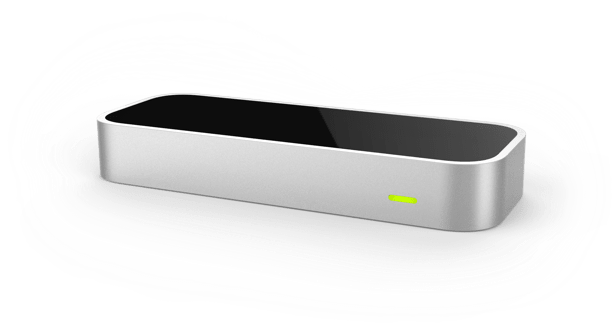
\includegraphics[width=\textwidth]{leap-motion}
	\end{subfigure}
	\begin{subfigure}{.3\textwidth}
		\center
		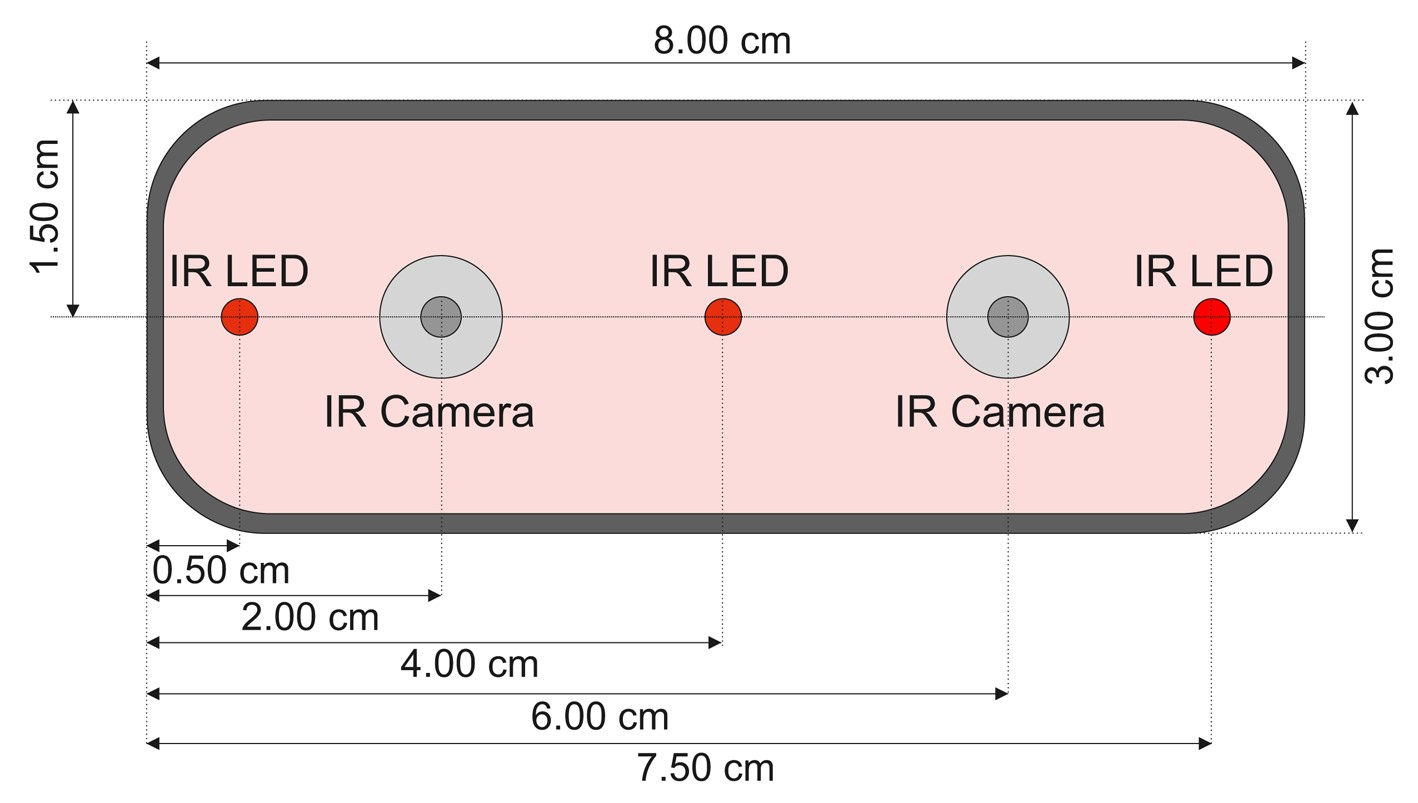
\includegraphics[width=\textwidth]{leap-motion-components}
	\end{subfigure}
	\begin{subfigure}{.3\textwidth}
		\center
		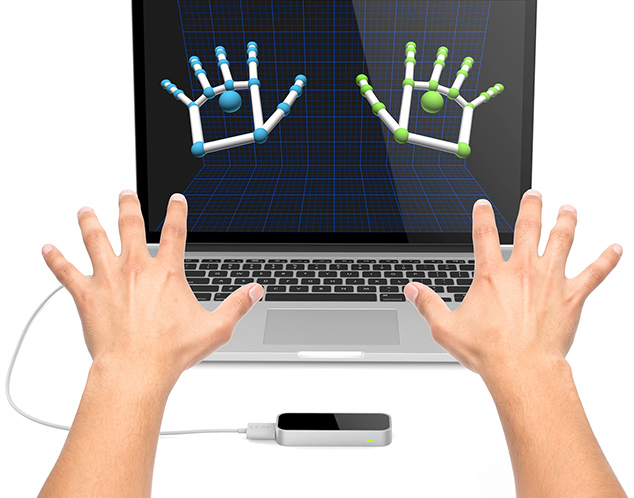
\includegraphics[width=\textwidth]{leap-motion-usage}
	\end{subfigure}
	\caption{Leap Motion Controller, sensors \protect\cite{leap-motion-components-image} and usage}
	\label{fig:leap-motion-components}
\end{figure}

\subsection{Kinect}\label{subsec:kinect}
The Microsoft Kinect is probably one of the best known and most widely used depth sensors.
It exists in two versions, which use different technologies to measure depth.
The first version of the Kinect used structured infrared light technology to create a depth map with a
resolution of $640 \times 480$ pixels and a frequency of 30 FPS~\cite{kinect-v1-and-v2-technical-info},
while the second version, the Kinect v2, uses a ToF sensor with a resolution of $512 \times 424$
pixels~\cite{kinect-v1-and-v2-technical-info} and a frequency of 30 FPS~\cite{kinect-v2-fps}.

The Kinect was originally designed for the Xbox 360 gaming console, but quickly became a popular
tool in research and development of interactive applications due to its ability to track human
body movements in real time and the dual presence of an infrared depth sensor and an RGB camera.

The Kinect has found applications in many areas beyond the video game industry, including
education~\cite{kinect-power-point, kinect-engineering, kinect-manipulation-3D-objects},
robotics~\cite{kinect-robot-1, kinect-robot-2},
and surveillance~\cite{kinect-surveillance-1, kinect-surveillance-2}.

\begin{figure}[ht]
	\begin{subfigure}{.5\textwidth}
		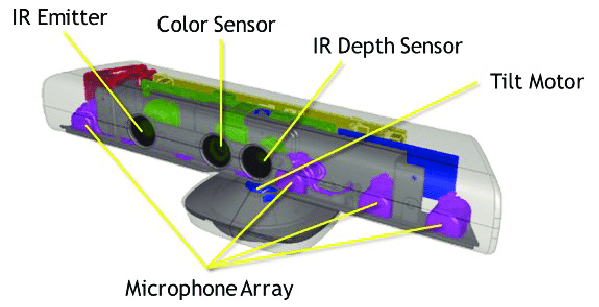
\includegraphics[width=\textwidth]{kinect-components}
	\end{subfigure}
	\begin{subfigure}{.5\textwidth}
		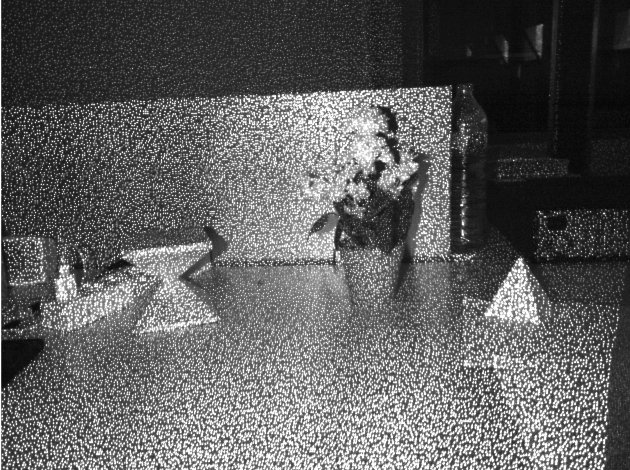
\includegraphics[width=\textwidth]{structured-light-kinect}
	\end{subfigure}
	\caption{Microsoft Kinect components \protect\cite{kinect-components-image} and structured light pattern \protect\cite{structured-light-kinect}}
	\label{fig:kinect-components}
\end{figure}

\subsection{RealSense}\label{subsec:realsense}
Intel's RealSense sensor line uses a combination of technologies,
including stereo vision and ToF, to provide high-resolution depth data.
RealSense sensors are designed to be integrated into a wide range of devices,
from drones to robots to AR and VR devices, thanks in part to the robust SDK developed by Intel,
which facilitates integration and custom application development.

RealSense sensors capture both depth images,
with a resolution of up to $1280 \times 720$ pixels and a frame rate of 90 FPS~\cite{realsense-resolution},
and RGB images, with a resolution of up to $1920 \times 1080$ pixels and a frame rate of 30 FPS~\cite{realsense-resolution}.

The ability of RealSense sensors to capture detailed depth maps makes them
ideal for 3D mapping applications even in outdoor environments~\cite{realsense-mapping}.
Among other fields of application, RealSense sensors are widely used in face detection
and its applications such as facial expression recognition~\cite{realsense-expressions},
3D face reconstruction~\cite{realsense-face-reconstruction},
and face detection~\cite{realsense-face-detection}.

\begin{figure}[ht]
	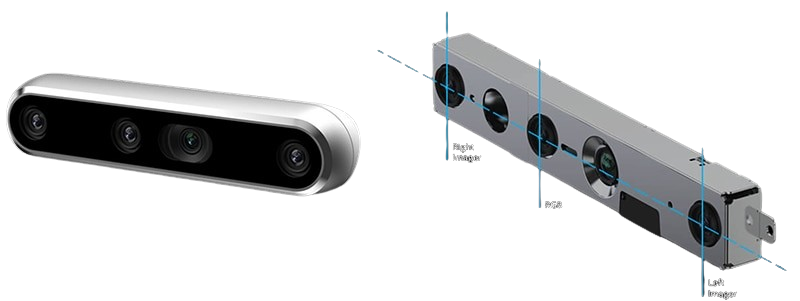
\includegraphics[width=\textwidth]{realsense}
	\caption{RealSense components}
	\label{fig:realsense-components}
\end{figure}




\section{Depth vision on smartphone}\label{sec:depth-vision-on-smartphone}
With the advent of smartphones equipped with powerful sensors and advanced cameras,
depth sensing has become accessible and usable in numerous applications.
It is mainly used in smartphones as an aid to the camera, to capture additional
information about the scene being framed and to improve sharpness and focus in photographs,
but it can also be used outside of simple photography apps, such as in augmented reality apps.

\subsection{Depth sensors on smartphone}\label{subsec:depth-sensors-on-smartphone}
Modern smartphones are often equipped with depth sensors that exploit different technologies,
such as LiDAR (Light Detection and Ranging) and ToF (Time-of-Flight).
These sensors calculate the distance to objects by emitting a light or laser pulse and measuring the
time it takes for it to return to the sensor after hitting an object.

\paragraph{LiDAR}
It uses laser pulses to create three-dimensional maps of the environment.
It is particularly useful in low light conditions and provides highly accurate depth data.
It can also measure the direction and intensity of the reflected signal,
providing three-dimensional information on the shape and structure of objects.
In smartphones, LiDAR greatly enhances AR capabilities, enabling more realistic and interactive applications.
This type of sensor can be found on Pro and Pro Max models of iPhone since the iPhone 12.

\paragraph{ToF}
It works similarly to LiDAR, but uses infrared light instead of a laser pulse to measure distance.
This type of sensor is often cheaper and less accurate
than LiDAR and does not provide information about the shape of objects,
but is still effective for many applications, including indoor mapping and object detection.

\subsection{ARFoundation for AR applications}\label{subsec:arfoundation-for-ar-applications}
ARFoundation is a Unity framework that enables developers to create cross-platform AR applications.
By integrating the functionality of Apple's ARKit and Google's ARCore, ARFoundation makes it possible
to develop a single application that can run on both iOS and Android devices.

\paragraph{Cross-platform}
One of the main features of ARFoundation is its ability to abstract the API
specifications of ARKit and ARCore, allowing developers to write code once to run applications on both platforms.
This reduces development time and simplifies code maintenance.

\paragraph{Detection and tracking}
ARFoundation supports tracking the position and orientation of the device, detecting horizontal and
vertical surfaces, anchoring virtual objects in real space and detecting 3D images and objects,
all essential functionalities for creating immersive and interactive AR experiences.

\subsection{Applications}\label{subsec:applications}
The use of sensors to detect depth images with a smartphone is applied in various fields,
from object detection and tracking, to health monitoring and assisting visually impaired people.

In~\cite{real-time-sign-language-translation}, the smartphone is used as a real-time sign language translator.
Depth images collected by the smartphone's depth sensor are pre-processed
and then classified by a MobileNet+LSTM deep-learning model directly on the mobile device.

Another tool of assistance for visually impaired people can be found in~\cite{smartphone-visual-assistance-system},
where a new solution for spatial orientation and navigation is proposed.
In this work the authors make use of techniques for distance detection and object recognition from RGB images,
using the MiDaS 2 Lite model to extrapolate a depth map and the MobiNet3 neural network for object classification.

Similar to the previous work, an object recognition system is proposed in~\cite{object-detection-using-smartphone},
but this time based on the depth sensor of the smartphone and not on RGB images.

A remarkable result was obtained in~\cite{smartphone-depth-for-medical-applications},
where the TrueDepth scanner of an iPhone 12 Pro was used to obtain a depth scan of
a stoma model in order to detect its contours, achieving a remarkable accuracy (<2mm).
In fact, it turns out that the TrueDepth scanner has a higher
accuracy and density of infrared dot projection than the LiDAR sensor.

However, it should be noted that the TrueDepth scanner is the one used
for FaceID and is located on the front face of the smartphone,
which makes it unusable together with the camera or any other sensor located on the back face of the smartphone.


\section{Hand detection}\label{sec:hand-detection}
With the advent of the era of augmented reality and virtual reality, the demand for virtual or semi-virtual interfaces
that do not require physical hardware to be used is growing more and more, and one of the most common methods of using
these interfaces is through the use of the hands, the most natural way we have of interacting with our surroundings.

In order to develop these types of interfaces so that they are reliable and comfortable to use,
there is a need for precise methods for detecting hands in a two- or three-dimensional space,
which can understand their positioning and interpret their gestures.

\subsection{MediaPipe}\label{subsec:mediapipe}
MediaPipe is an open-source framework developed by Google for multimodal processing of data streams.
Its flexibility and power make it an ideal tool for developing virtual reality and augmented reality applications.
MediaPipe allows the creation of modular pipelines that can be used in various applications such as facial recognition,
object tracking, hand detection and many others.

\subsubsection{Origin and history}
MediaPipe started as an internal solution to manage and standardise the various computer vision algorithms used in their products.
In 2019~\cite{mediapipe}, Google decided to make MediaPipe an open-source project,
allowing the developer community to contribute and exploit the potential of the platform.
Since its release, MediaPipe has seen rapid adoption due to its ability to simplify development.

\subsubsection{Components and architecture}
MediaPipe's architecture is based on a modular design that allows developers to combine various components to create customised pipelines.
The main components of MediaPipe include:
\begin{itemize}
	\item \textit{Calculator:} it is the fundamental unit of calculation that perform specific operations on data.
	Each calculator receives an input, processes the data and produces an output.
	\item \textit{Graph:} it is a network of calculators that defines the flow of data.
	The graph determines how the data is transformed and transferred between the various calculators.
	\item \textit{Packet:} it is the data transport unit in the graph.
	Packets may contain any type of data, such as images, videos or processing results.
	A particular type of packet is the side packet, a packet without a timestamp that can be used to transport data
	that remain constant, unlike a stream that represents a flow of data that changes over time.
\end{itemize}

\paragraph{Pipeline}
A MediaPipe pipeline is essentially a graph of calculators.
This modular design allows the construction of highly customisable pipelines.
For example, a hand detection pipeline may include calculators for image pre-processing,
hand detection, tracking of key points and post-processing of results.
MediaPipe provides a number of predefined calculators,
but developers can also create their own calculators~\cite{calculators-can-be-created} for specific application needs.
The main components of MediaPipe are:
\begin{itemize}
	\item \textit{Input Streams:} these are sources of data such as video feeds, audio inputs, or sensor data.
	\item \textit{Processing Nodes:} these nodes perform specific tasks like image transformation, feature extraction,
	and machine learning model inference.
	\item \textit{Output Streams:} the processed data is outputted for use in applications,
	such as displaying detected hand gestures or controlling a robotic arm.
\end{itemize}

\paragraph{Hand recognition}
One of the most advanced and popular features of MediaPipe is hand recognition~\cite{mediapipe-hands}.
This feature is designed to be accurate and fast,
working in real time even on mobile devices~\cite{mediapipe-lens-characteristics, mediapipe-sign-language}.
MediaPipe's hand recognition pipeline consists of several steps:
\begin{itemize}
	\item \textit{Hand Detection:} it uses a machine learning model to identify the presence of hands in an image.
	This model is optimised to identify hands in various positions and orientations.
	\item \textit{Landmarks Localization:} once the hand is detected,
	another machine learning model tracks 21 specific landmarks of the hand,
	which include the positions of the finger and palm joints in 2.5D\@.
	The landmarks used by MediaPipe are shown in \autoref{fig:mediapipe-hand-landmarks}
	\item \textit{Post-Processing:} landmark data can be further processed for specific applications,
	such as gesture recognition or interaction with virtual user interfaces.
\end{itemize}
MediaPipe's hand detection model has been trained on a large dataset to ensure high accuracy and robustness.
The pipeline is optimised to run in real time, making it suitable for interactive applications such as
augmented reality games and gesture-based controls.

\begin{figure}[ht]
	\centering
	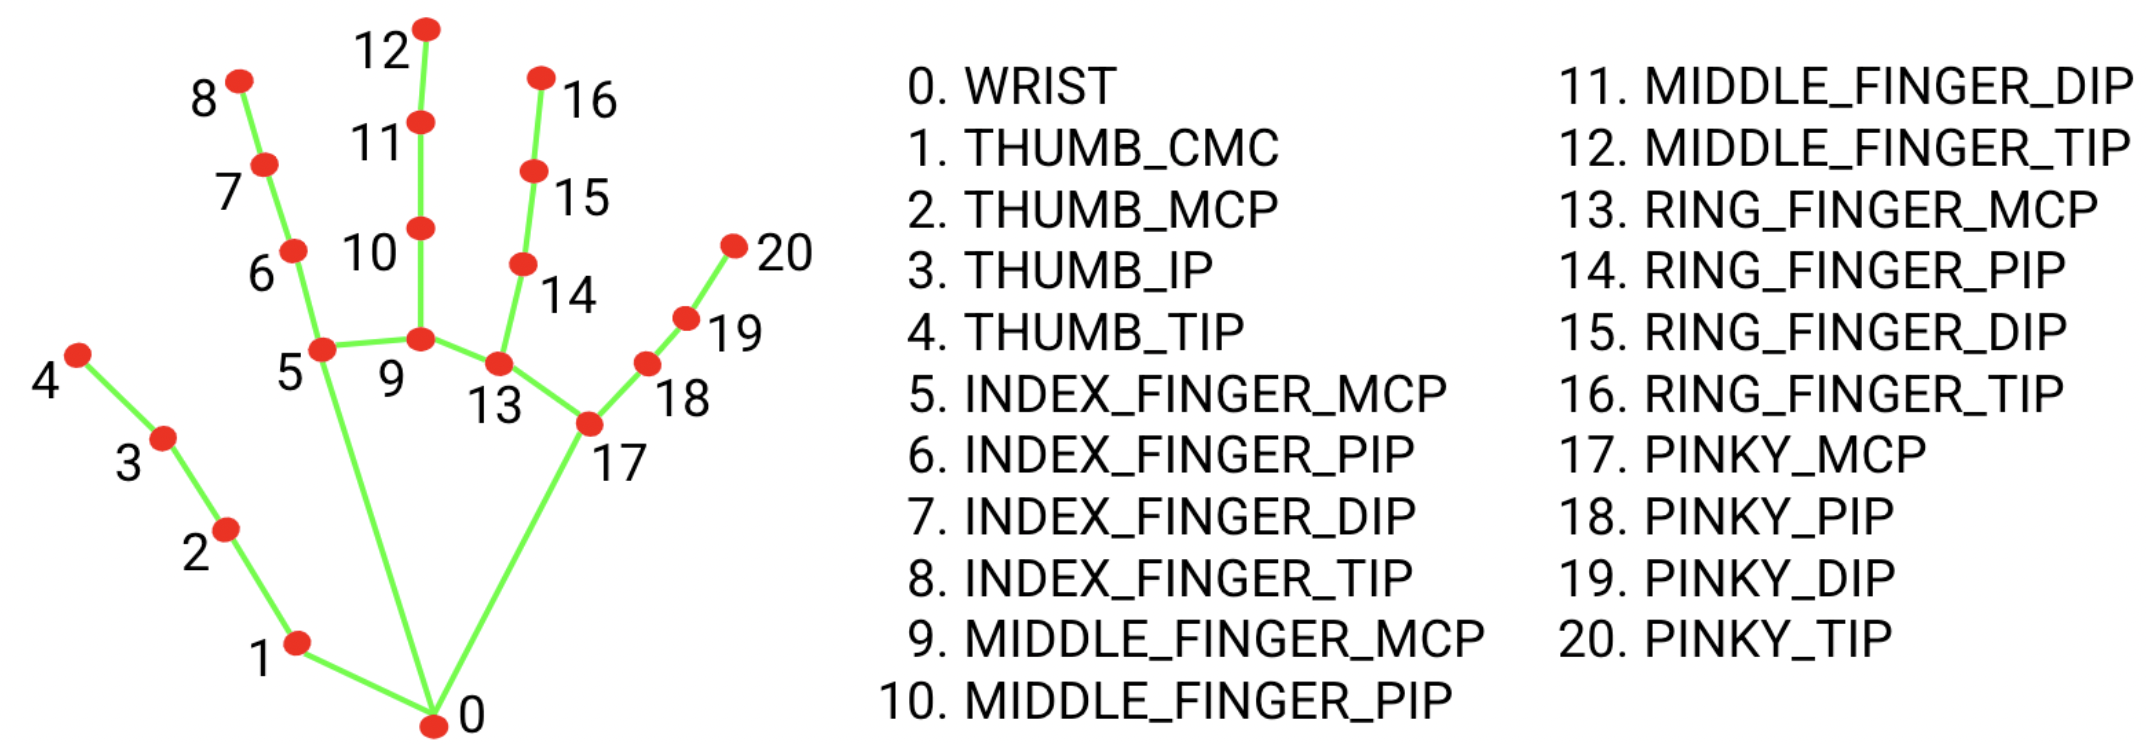
\includegraphics[width=\textwidth]{mediapipe-hand-landmarks}
	\caption{MediaPipe Hand Landmarks}
	\label{fig:mediapipe-hand-landmarks}
\end{figure}

\subsection{ManoMotion}\label{subsec:manomotion}
ManoMotion is an advanced hand gesture recognition technology that fits into the field of augmented reality and virtual reality.
Founded in 2015, ManoMotion's main goal is to provide intuitive and natural interaction between humans
and digital devices through real-time detection of hand movements.

\paragraph{Features}
ManoMotion offers several advanced features that make its hand gesture detection technology particularly useful:

\begin{itemize}
	\item \textit{3D movement recognition:} the technology is able to track hand movements in three dimensions,
	detecting not only the position, but also the depth and orientation of the hands.
	\item \textit{Complex gesture recognition:} ManoMotion can recognise a wide range of complex gestures,
	including finger movements, grasps and releases, rotations and more.
	\item \textit{AR and VR integration:} ManoMotion is designed to easily integrate with leading AR and VR development
	platforms, such as Unity and AR Foundation, facilitating adoption by developers.
	\item \textit{Real-time analysis:} ManoMotion's algorithms process data in real time,
	ensuring a smooth interaction with no perceptible delays.
	\item \textit{Compatibility with mobile devices:} one of the main innovations of ManoMotion is the ability
	to operate on mobile devices, using standard cameras built into phones and tablets.
\end{itemize}

\paragraph{Smartphone}
The way ManoMotion works on a smartphone is particularly impressive: it relies on a remote computing system
in which the smartphone continuously sends the camera's video stream to the ManoMotion server,
which then performs hand and gesture recognition and sends them back to the smartphone in real time.

This method involves shifting the computational load from the smartphone to the ManoMotion servers,
leaving the smartphone with the sole task of transmitting the video stream to the server.
ManoMotion certainly requires a stable and fairly fast connection
(note that the frames sent by the smartphone are not in high resolution anyway),
but it results in a huge reduction in computational load on the part of the smartphone.

This makes ManoMotion particularly suitable for the development of educational applications,
thus intended to be in a classroom, where a school Wi-Fi could be available for use.
An example is the work done in~\cite{manomotion-agilest},
in which ManoMotion is used to create an educational application for chemistry.
This application uses real-time touchless interaction for
kinesthetic and machine learning with a dual purpose: teacher and student evaluator.

\begin{figure}[ht]
	\centering
	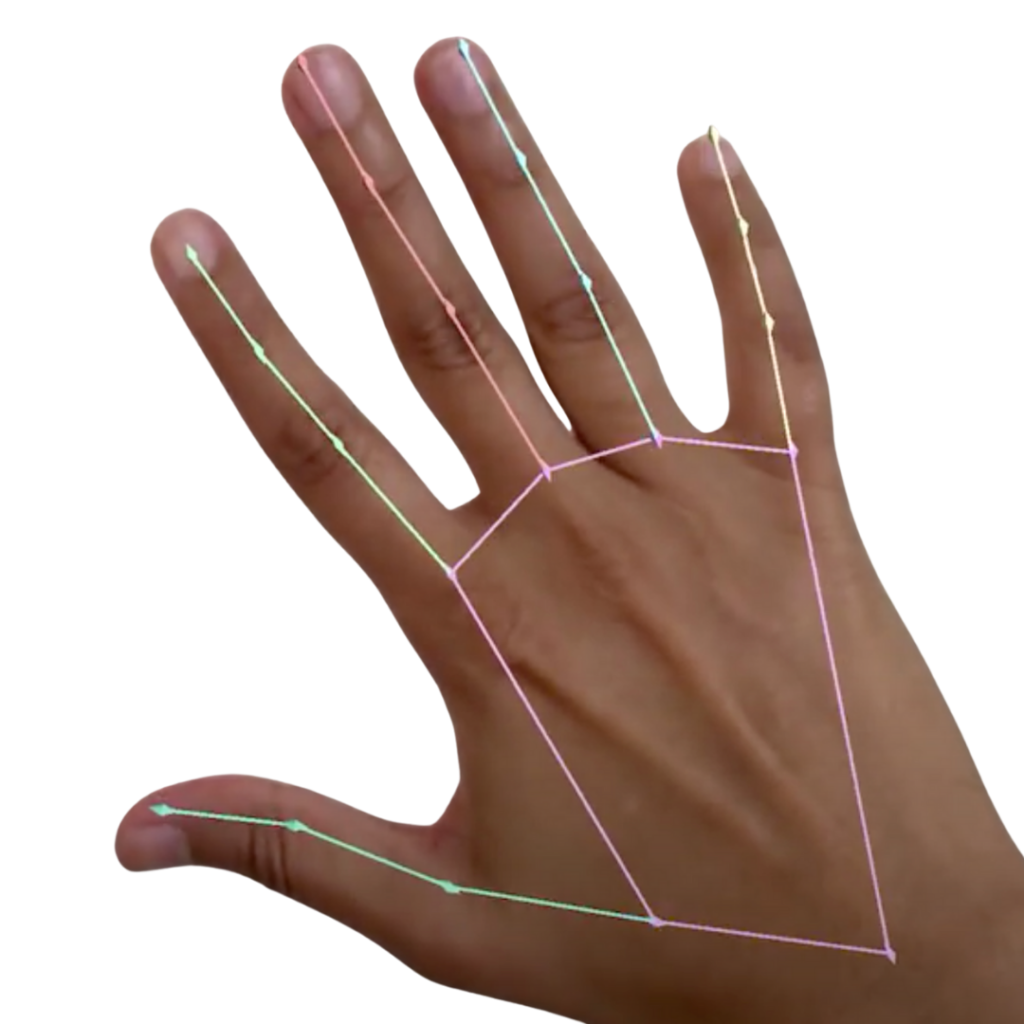
\includegraphics[width=0.5\textwidth]{manomotion-hand}
	\caption{ManoMotion hand skeleton}
	\label{fig:manomotion}
\end{figure}


\section{Related work}\label{sec:related-work}
There are many software and technologies that bring music into virtual reality or augmented reality applications,
from systems for playing virtual or semi-virtual instruments,
to virtual tutors evaluating the musical performance of a beginner musician.

\subsection{Virtual and semi-virtual instruments}\label{subsec:virtual-and-semi-virtual-instruments}
One of the most important features of VR and AR is to make the user interface with something that does not exist,
but at the same time is visible in a virtual or semi-virtual environment, with even the possibility of giving feedback
visual or tactile feedback in response to an action.

In~\cite{cyber-glove} Cyber Composer is proposed, an interactive cyber instrument to enable both musicians and music laypersons
to dynamically control the tonality and the melody of the music that they compose through hand motion and gestures.
This system is empowered by the embedding of music theories to ensure the music
generated makes musical sense in the perspective of musicians.

Two sensors are used to track hand movements: a pair of CyberGlove and a Polhemus FASTRAK 3D Position Tracker.
The CyberGlove provides high-performance hand measurements and real-time motion capture
thanks to bend and flexion sensors on fingers, palm, and wrist.
A Polhemus sensor is attached to each glove, to provide 3D positioning and orientation information.

The software consists of four components:
music interface, CyberGlove interface, background music generation module and melody generation module,
all linked together by the main program, which provides a user-friendly graphical user interface.

The system implements seven musical expressions, mapping each one to a different kind of motion of gesture with one or two hands.
The musical expressions are rhythm, pitch, pitch-shifting, dynamics, volume, dual instrument mode, and cadence.
The gestures used to control the generated melody include, among others, flexion of the right wrist,
height of the right hand relative to the ground and lifting of the same hand,
position of the left hand relative to the right hand, and bending the fingers of the left hand.

\begin{figure}[ht]
	\centering
	\begin{subfigure}{0.32\textwidth}
		\centering
		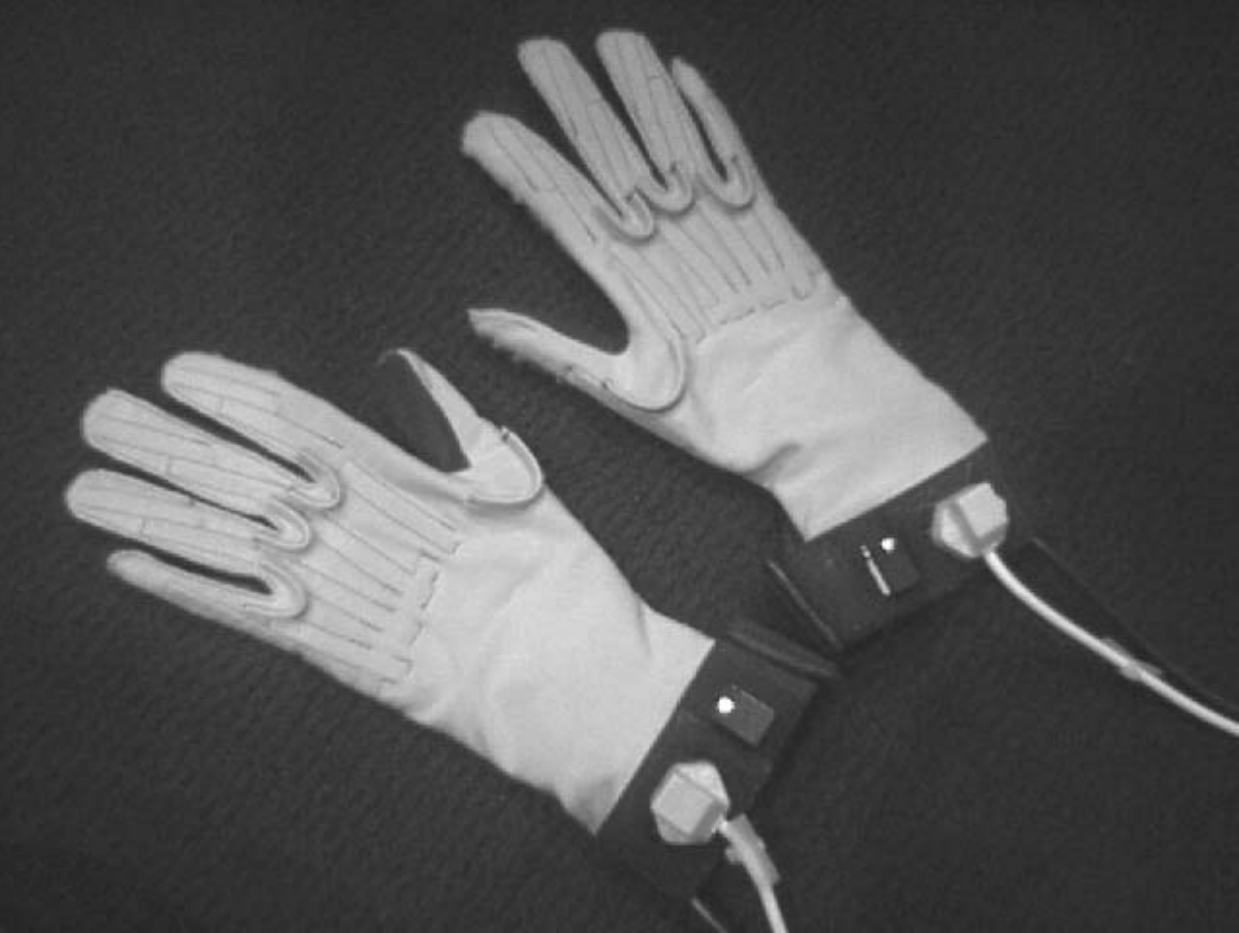
\includegraphics[width=\textwidth]{images/related-work/cyber-gloves}
	\end{subfigure}
	\hfill
	\begin{subfigure}{0.32\textwidth}
		\centering
		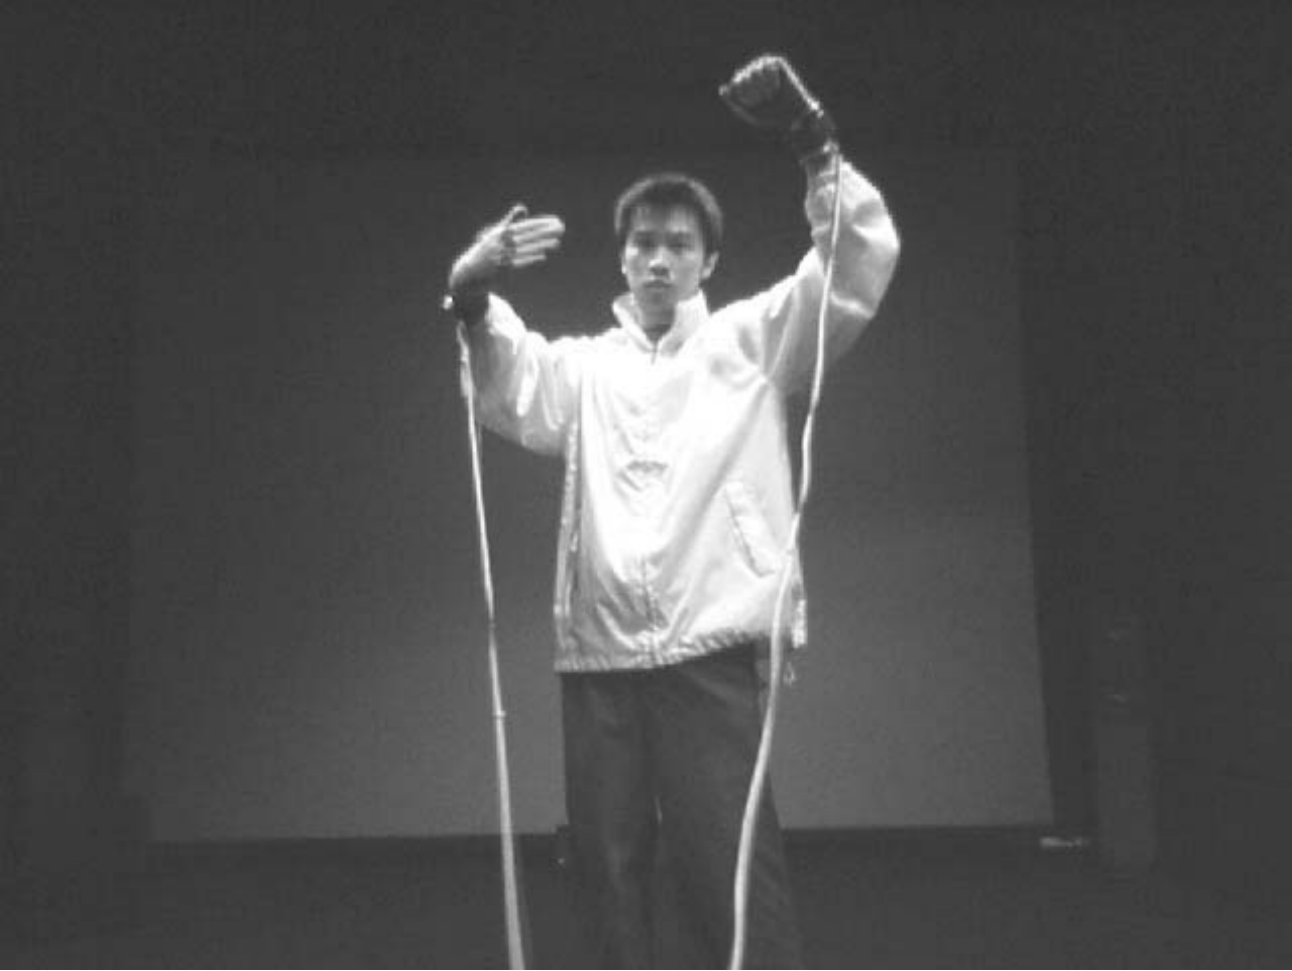
\includegraphics[width=\textwidth]{images/related-work/cyber-gloves-example}
	\end{subfigure}
	\hfill
	\begin{subfigure}{0.32\textwidth}
		\centering
		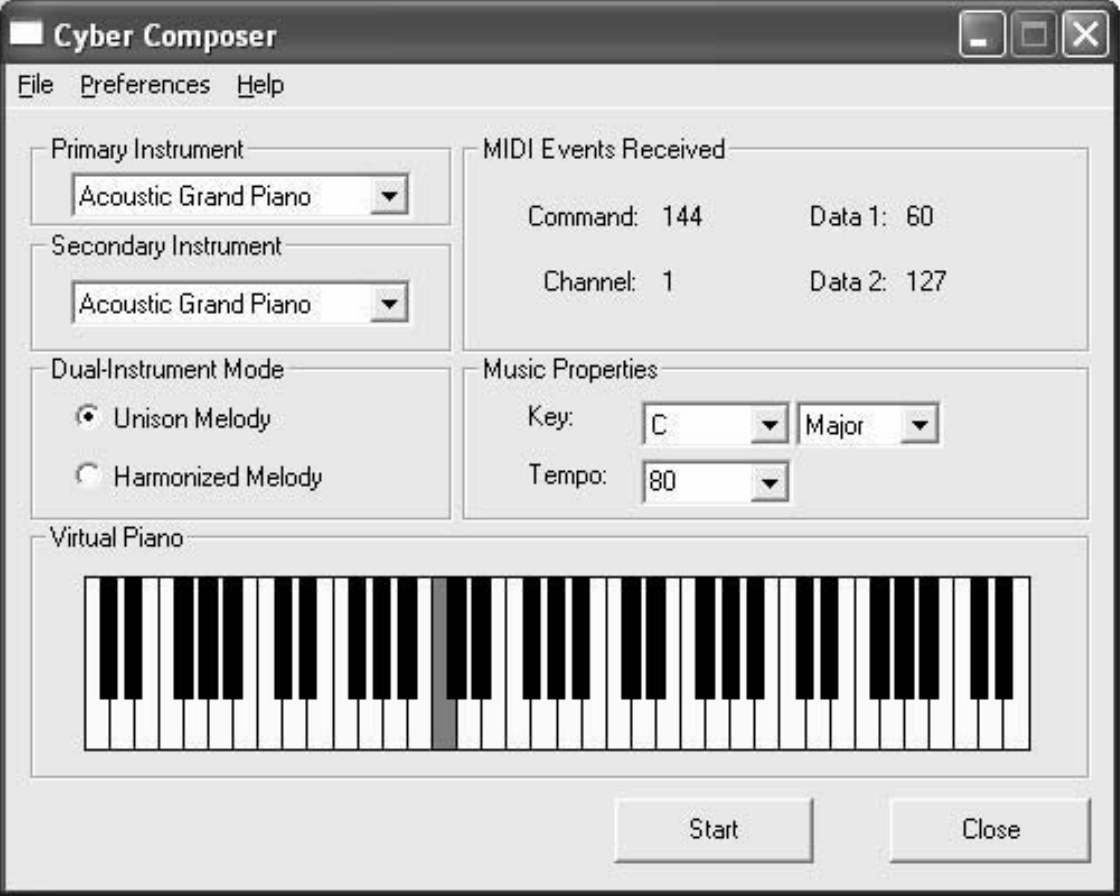
\includegraphics[width=\textwidth]{images/related-work/cyber-glove-gui}
	\end{subfigure}
	\caption{CyberGloves used in Cyber Composer~\protect\cite{cyber-glove} and its graphical user interface}
	\label{fig:cyber-glove}
\end{figure}

In~\cite{semi-virtual-instruments} two semi-virtual instruments based on physical interfaces are implemented:
a flute and a drum.

A semi-virtual flute is created using a real plastic tube with three buttons and a small fan inside,
which is activated by the user's breath.
The rotation of the fan is transmitted to the computer, which processes it together with the data on the buttons pressed,
producing the corresponding sound.
A drum, on the other hand, is created using only a stick with a red object attached to the tip.
The red tip is tracked by the webcam, which calculates its movement by keeping track of its position and speed.

Both the flute and the drum can be visualized live on the computer screen, accompanied by visual effects
which inform the user of the type of sound produced.

\begin{figure}[ht]
	\centering
	\begin{subfigure}{0.32\textwidth}
		\centering
		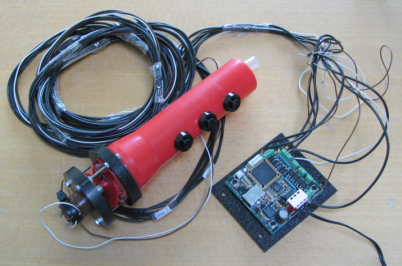
\includegraphics[width=\textwidth]{images/related-work/semi-virtual-flute}
	\end{subfigure}
	\hfill
	\begin{subfigure}{0.32\textwidth}
		\centering
		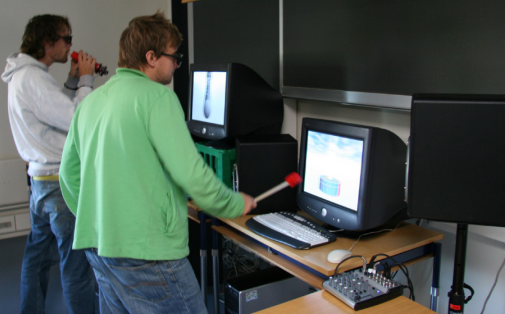
\includegraphics[width=\textwidth]{images/related-work/semi-virtual-drum}
	\end{subfigure}
	\hfill
	\begin{subfigure}{0.32\textwidth}
		\centering
		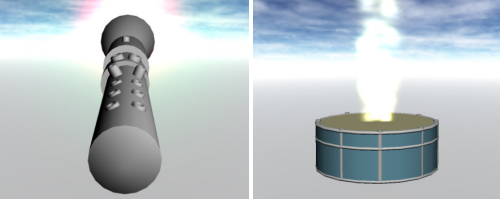
\includegraphics[width=\textwidth]{images/related-work/semi-virtual-visualization}
	\end{subfigure}
	\caption{Semi-virtual flute, semi-virtual drum and their visualization in~\protect\cite{semi-virtual-instruments}}
	\label{fig:semi-virtual}
\end{figure}

In~\cite{hand-gesture-controlled-music-instrument}, a system is developed to play a virtual instrument
using hand gestures to modify its parameters such as pitch name, octave, accidentals, instrument
pitch bend, note value, and frequency equalizer.

Pitch, octave and accidentals are controlled with the right hand.
The number and position of the fingers bent towards the palm are used to distinguish pitch, while
the position of the palm in relation to the shoulder is used to control octave and accidentals.
The left hand is used to control the type of instrument (trumpet or piano) and the pitch bend using three movement actions.
Based on the angle of both hands, the note value and frequency can be controlled.

This system works in both real-time and delayed mode, achieving an accuracy of 90.8\% and 98.85\% respectively.

\begin{figure}[ht]
	\centering
	\begin{subfigure}{0.32\textwidth}
		\centering
		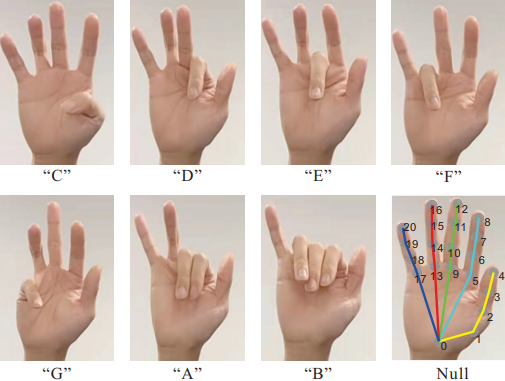
\includegraphics[width=\textwidth]{images/related-work/pitch-control}
	\end{subfigure}
	\hfill
	\begin{subfigure}{0.32\textwidth}
		\centering
		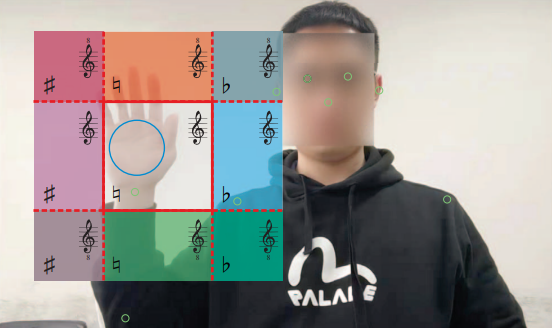
\includegraphics[width=\textwidth]{images/related-work/octave-control}
	\end{subfigure}
	\hfill
	\begin{subfigure}{0.32\textwidth}
		\centering
		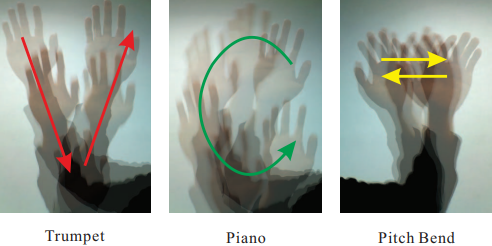
\includegraphics[width=\textwidth]{images/related-work/instrument-control}
	\end{subfigure}
	\caption{Instrument controls from~\protect\cite{hand-gesture-controlled-music-instrument}}
	\label{fig:instrument-control}
\end{figure}

In~\cite{emg-midi-controller}, an EMG based MIDI controller is implemented and tested.
The controller needs both a complex physical architecture and an intricate software to run.
The purpose of the controller is to identify four hand gestures, each associated with a different note.

The hardware consists of four components:
three EMG (Olimex Shield-EKG-EMG) sensors to be connected to the arm that is to act as the controller,
an Arduino UNO board to read the data from the three EMG sensors,
a Raspberry PI 4B board to receive the data from the Arduino and interpret it with the gesture recognition software,
and a computer that receives the final signal containing the MIDI note to be played.

The software communication between these devices is architected in the following way,
and is schematised in~\autoref{fig:emg-controller}.
First, the Arduino UNO board reads data from the three EMG sensors.
Then the Raspberry PI board requests this data from the Arduino, and when it receives it,
it passes it to the classifier that produces the hand gesture.
The result of the classifier is sento to the Arduino,
which converts it into a MIDI note and sends it to the computer so that the note can be played.

Three types of classifiers are used to test the system: Random Forest,
Support Vector Machines and a Neural Network with three hidden layers.
All three classifiers are trained on a dataset consisting of 60 measurements per each of the four gestures.

The results are unfortunately lower than hoped for,
with a maximum of 78\% obtained by SVM and a minimum of 71\% obtained by the Neural Network.
According to the authors, the cause for such a low result could be the Arduino,
which is deemed compromising for applications that require high sampling rates.

\begin{figure}[ht]
	\centering
	\begin{subfigure}{0.32\textwidth}
		\centering
		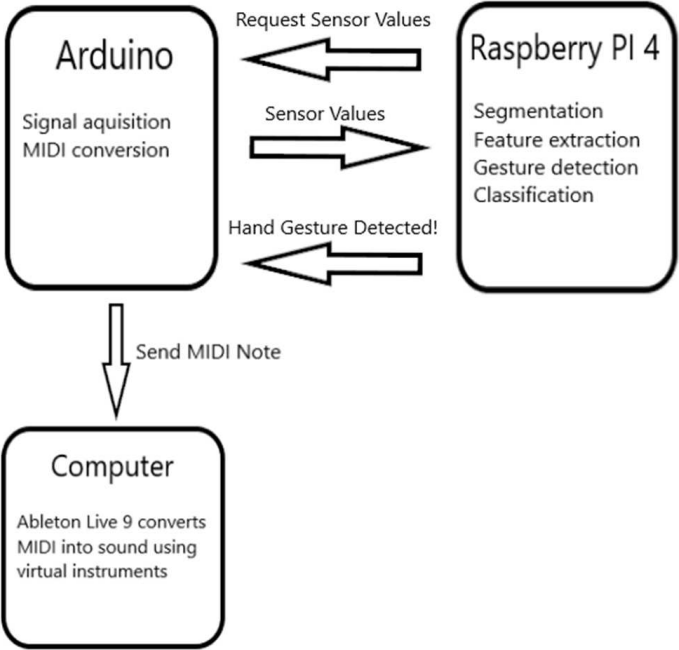
\includegraphics[width=\textwidth]{images/related-work/emg-architecture}
	\end{subfigure}
	\hfill
	\begin{subfigure}{0.32\textwidth}
		\centering
		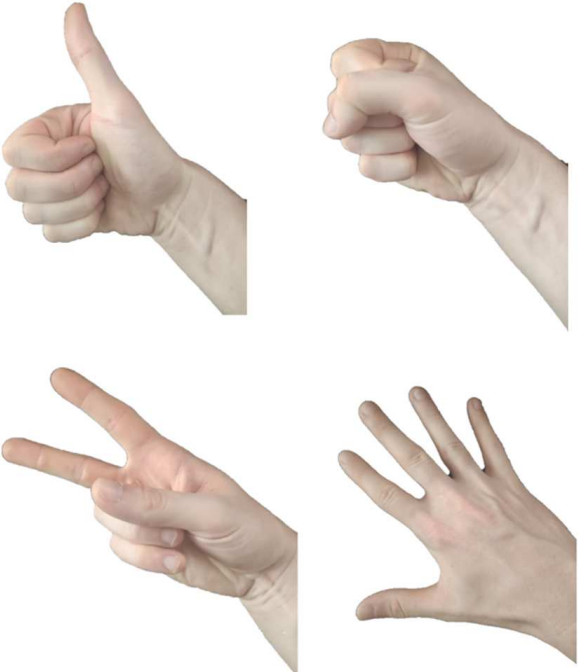
\includegraphics[width=\textwidth]{images/related-work/emg-gestures}
	\end{subfigure}
	\hfill
	\begin{subfigure}{0.32\textwidth}
		\centering
		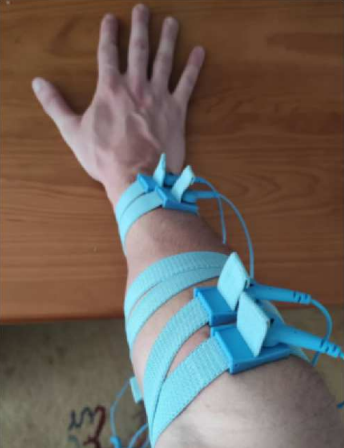
\includegraphics[width=\textwidth]{images/related-work/emg-sensors}
	\end{subfigure}
	\caption{Architecture, gestures and sensor position from~\protect\cite{emg-midi-controller}}
	\label{fig:emg-controller}
\end{figure}

\subsection{Virtual trainers}\label{subsec:virtual-trainers}
When it comes to learning a musical instrument using virtual reality tools,
it is not only important to have a tool that allows one to play
but also a tutoring system that gives feedback on the quality of the novice musician's performance.

The work done in~\cite{piano-fingering-recognition} is not exactly a virtual reality application, but still
represents an example of how depth sensors can be used for teaching and learning how to play a musical instrument.
This paper proposes a method for recognising piano fingering by analysing motion of multiple fingers through the use
of depth images acquired with a depth sensor.
The depth sensor used in the paper is a Microsoft Kinect, but in theory any other depth sensor may be used.

The proposed method consists of two modules: a learning module and a recognition module.
The learning module is used to generate a dataset of depth images for various key pressing patterns.
The recognition modules takes a depth image as input and tries the best matching key pressing pattern in the dataset,
with the goal to identify which one is being performed in the input depth image.
The recognition process uses the Nearest-Neighbor search technique.
Both the learning module and the recognition module make use of a background subtraction technique,
to separate the depth information about the keyboard from those about the hand.

The method was tested on three songs, with a dataset of 780 data elements in 130 classes acquired
by the learning module, obtaining a maximum recognition rate of 100\%, and a minimum of 91.6\%.
The recognition time was also measured and found to be 120 milliseconds per image,
making this method applicable to slow-tempo songs for piano beginners.

\begin{figure}[ht]
	\centering
	\begin{subfigure}{0.55\textwidth}
		\centering
		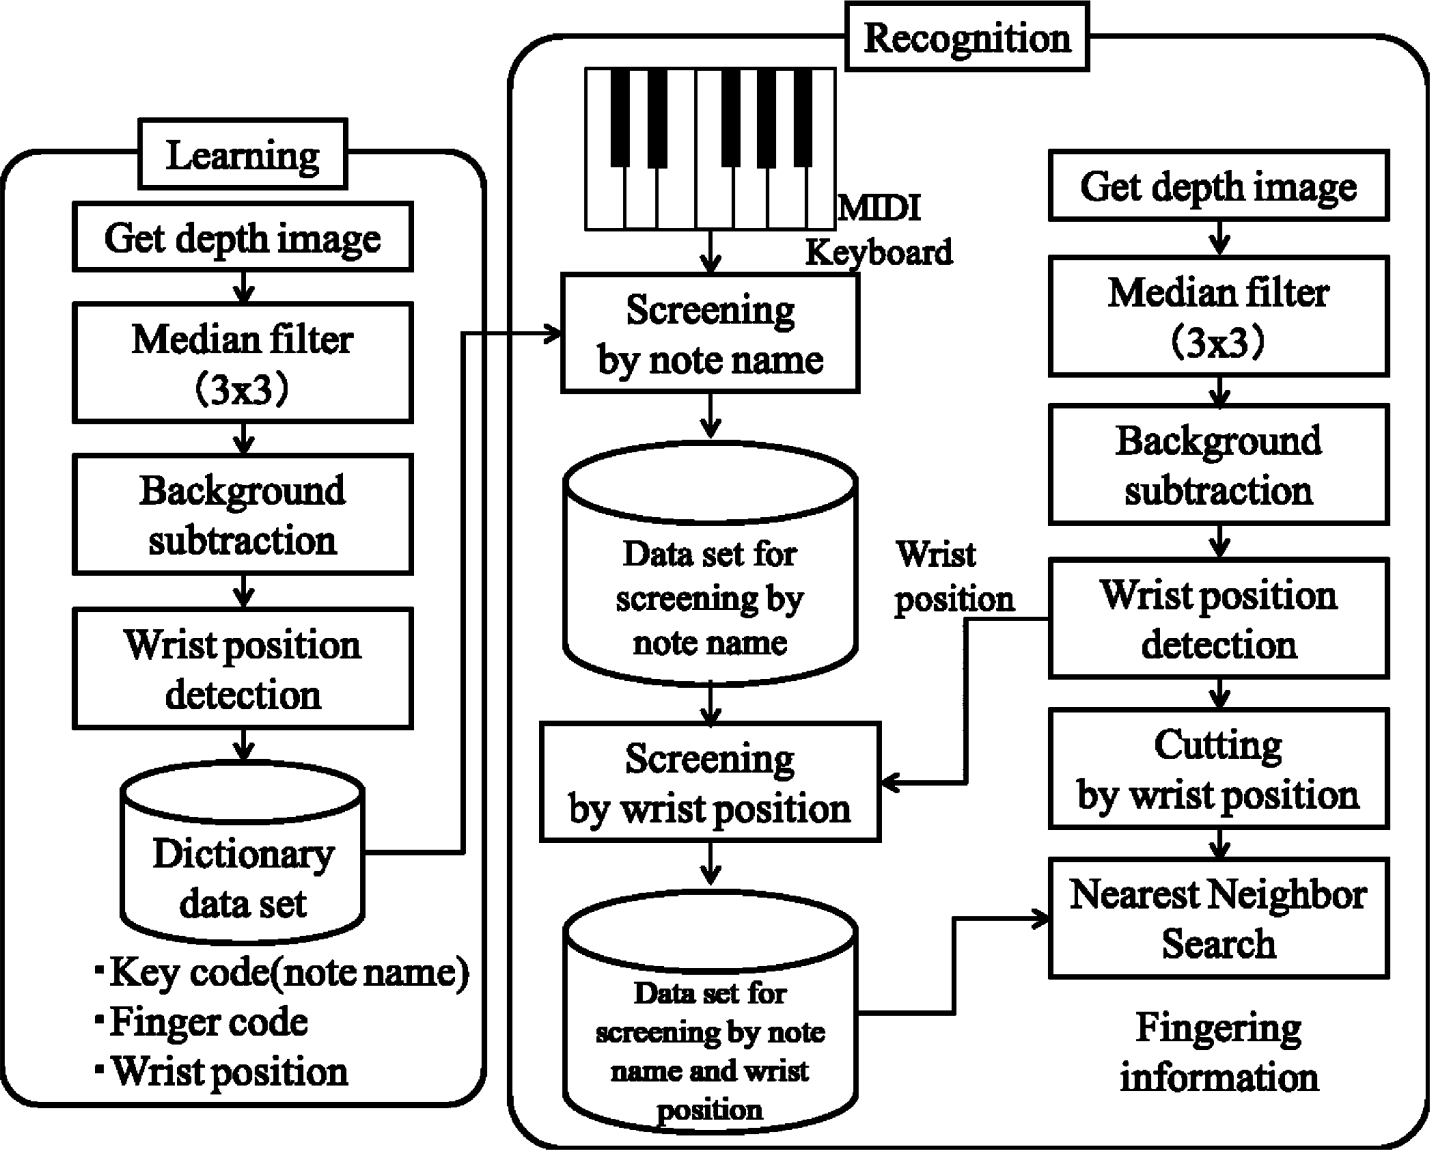
\includegraphics[width=\textwidth]{images/related-work/fingering-recognition-scheme}
	\end{subfigure}
	\hfill
	\begin{subfigure}{0.43\textwidth}
		\centering
		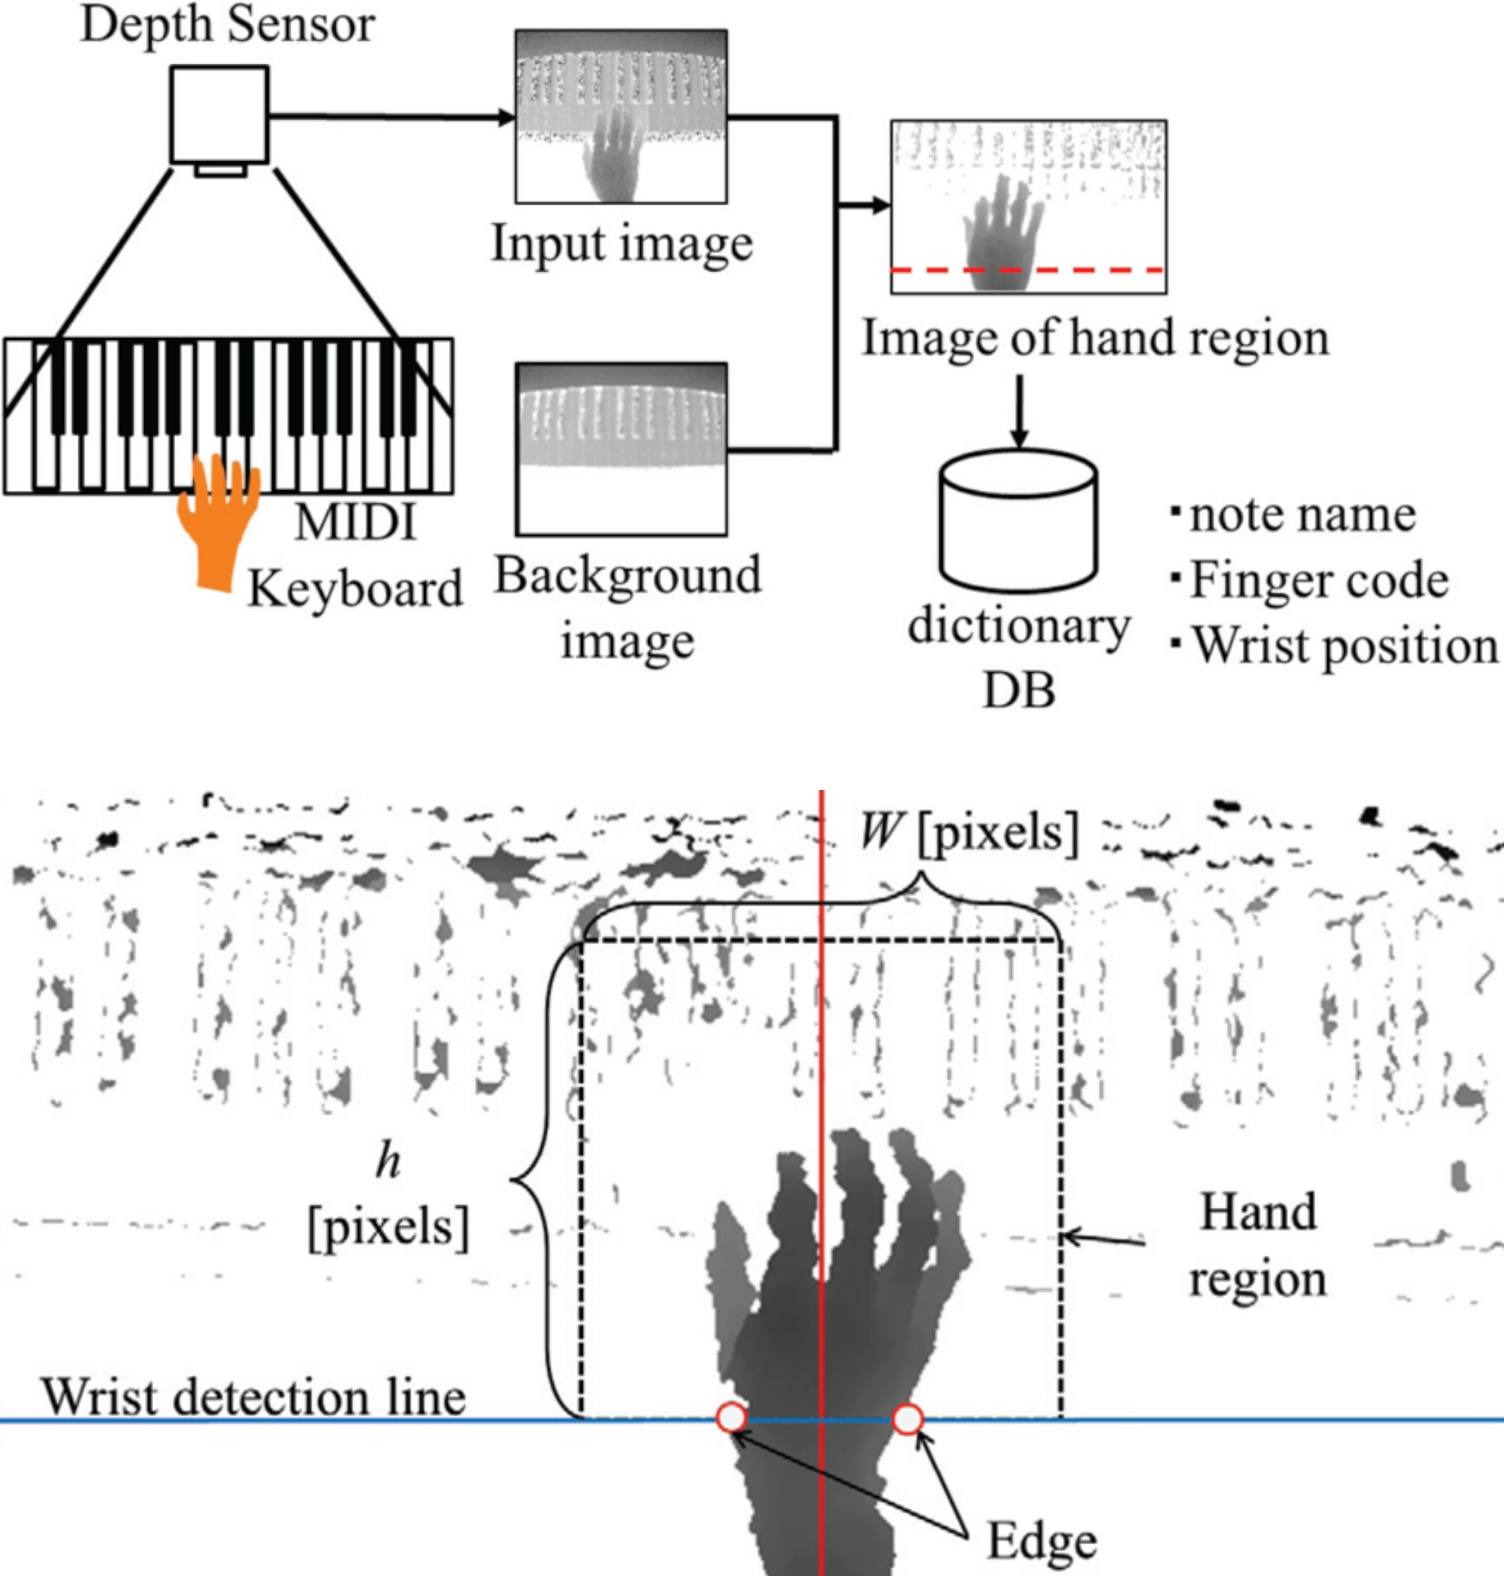
\includegraphics[width=\textwidth]{images/related-work/fingering-recognition}
	\end{subfigure}
	\caption{Architecture scheme, learning flow and recognition phase from~\protect\cite{piano-fingering-recognition}}
	\label{fig:fingering-recognition}
\end{figure}

In~\cite{fingering-generation}, an AR-based individual tutorial system is proposed.
Its goal is to automatically generate hand action animations
and displaying animations with real pianos using head-mounted displays.
Starting from a piece of music given as input, the system generates a coherent and natural-looking
animation of hands playing the given sequence of notes on a virtual piano.

To go from a MIDI file to an animation of hands playing a piano, two steps are taken.
The first step is to convert the raw MIDI file o a fingering-tagged MIDI file,
in which every note is tagged with the finger that plays it.
This is done with a Hidden Markov Model (HMM) and the Viterbi algorithm.
The HMM can be applied not only to single notes but also to chords that require a multi-finger movement.
The second step consists in creating the actual hand animation from the finger-tagged MIDI file.
The three patterns of fingering that can be recognised are Basic Finger Motion,
Alternative Finger Motion and Multi-finger Hand Motion.
To produce human-like animations for all these patterns,
the authors have defined step-by-step animations for each and every case above.

\begin{figure}
	\center
	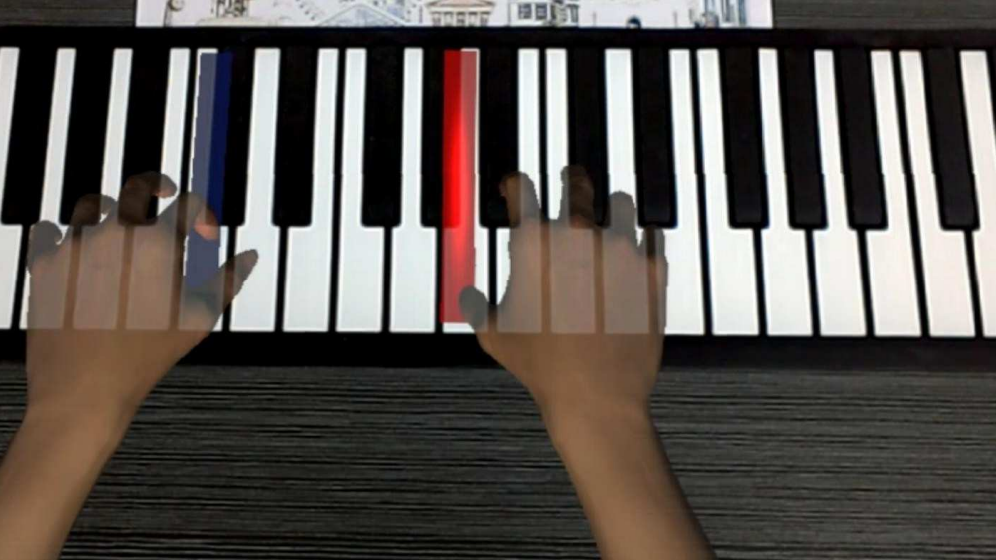
\includegraphics[width=0.7\textwidth]{images/related-work/fingering-generation}
	\caption{Fingering generation in an augmented reality environment from~\protect\cite{fingering-generation}}
	\label{fig:fingering-generation}
\end{figure}

Piano Beginner~\cite{piano-glove-training} is a finger training system with auditory and visual feedback (AVFB),
which supports both single-finger and multi-finger movements of two hands.
By wearing a pair of 5DT Data Glove Ultra and an optional VR headset, the user can experience an immersive simulation
of piano training.

The peculiarity of this project is in the setup phase:
rather than using a generic algorithm to detect finger pressure, the authors develop a calibration process
in which the user performs some actions like closing the hand and pressing each finger singularly,
to let the program learn what is the correct threshold to detect pressure for each finger.

The results of the experimentation show that users' accuracy increases by more than 20\% after 20 training sessions.

\begin{figure}[ht]
	\centering
	\begin{subfigure}{0.49\textwidth}
		\centering
		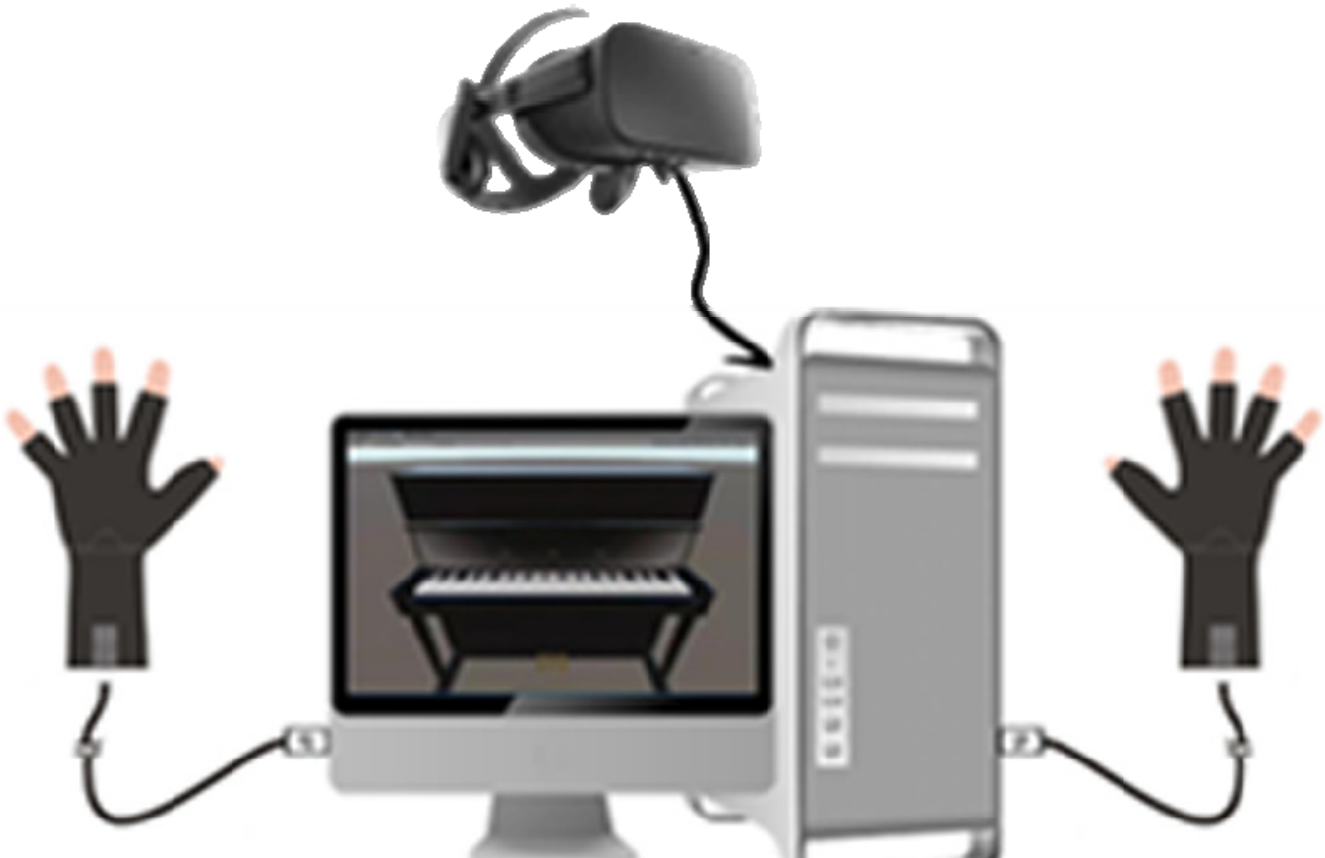
\includegraphics[width=\textwidth]{images/related-work/piano-glove}
	\end{subfigure}
	\hfill
	\begin{subfigure}{0.49\textwidth}
		\centering
		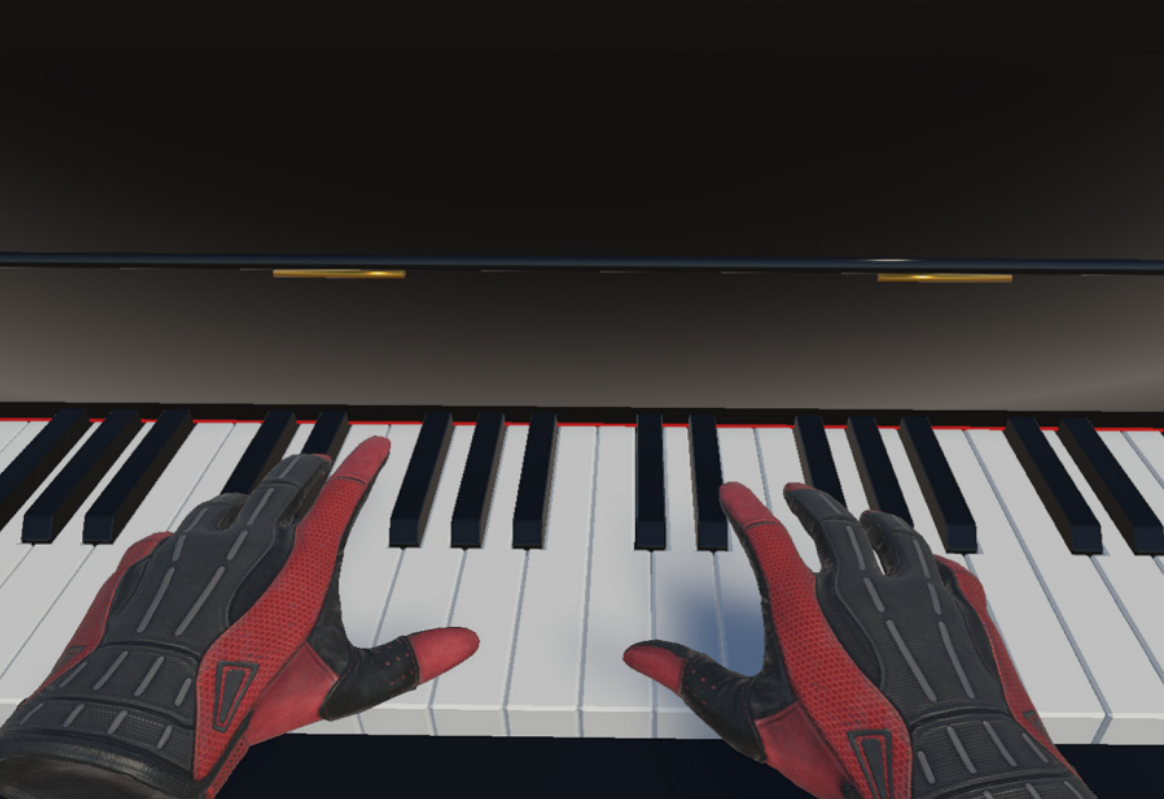
\includegraphics[width=\textwidth]{images/related-work/piano-glove-unity}
	\end{subfigure}
	\caption{Glove-based finger training system from~\protect\cite{piano-glove-training} and its Unity3D environment}
	\label{fig:piano-glove-training}
\end{figure}

GuitarGuru~\cite{guitar-guru} is a multi-featured application that caters for beginner guitarists with four
methods to learn and improve their performance on the guitar, combining computer vision and deep learning techniques.

The first feature allows a user to upload a video, or a link to a video on YouTube,
in which a musician plays the guitar.
GuitarGuru analyses the video and extracts all the chords from it in the form of a chord sheet.
With this function the user can also play the guitar in front of the webcam and get the chord sheets in real-time.

The second feature consists of a training session: the user selects a chord sheet from those previously
generated with the first feature, then starts the webcam and the application analyses their performance in real time,
evaluating its correctness and calculating the accuracy rate.

The third feature is similar to the previous but is a more specific and focused test on individual chords.
The user stands in front of the webcam and plays one chord at a time,
while the application measures the accuracy of each individual chord that is played.

The last feature is about music theory, offering a section where the beginner can learn notions about all the
music-related theories that will help the user in learning the basics of music,
including brief information about chords, scales, pitch, etc.

The dataset to train the deep learning model was built using python with OpenCV for preprocessing and MediaPipe for
extracting hand gestures, resulting in 25000 images: 5000 per each chord A, C, F, G, and 5000 representing a no-chord,
in which none of the previous chords was detected.
The deep learning model was built with Keras, with one input neuron and one output neuron,
32 filters in each layer and the size of a layer being (5, 5) with Relu as the activation function.

The model gives an accuracy of 97.09\% for the 4 chords A, C, F, G and a loss of 2.91\%.
In the future, more chords can be added for identification,
which would help expand the range of music genres to which GuitarGuru can be applied.

\begin{figure}[ht]
	\centering
	\begin{subfigure}{0.60\textwidth}
		\centering
		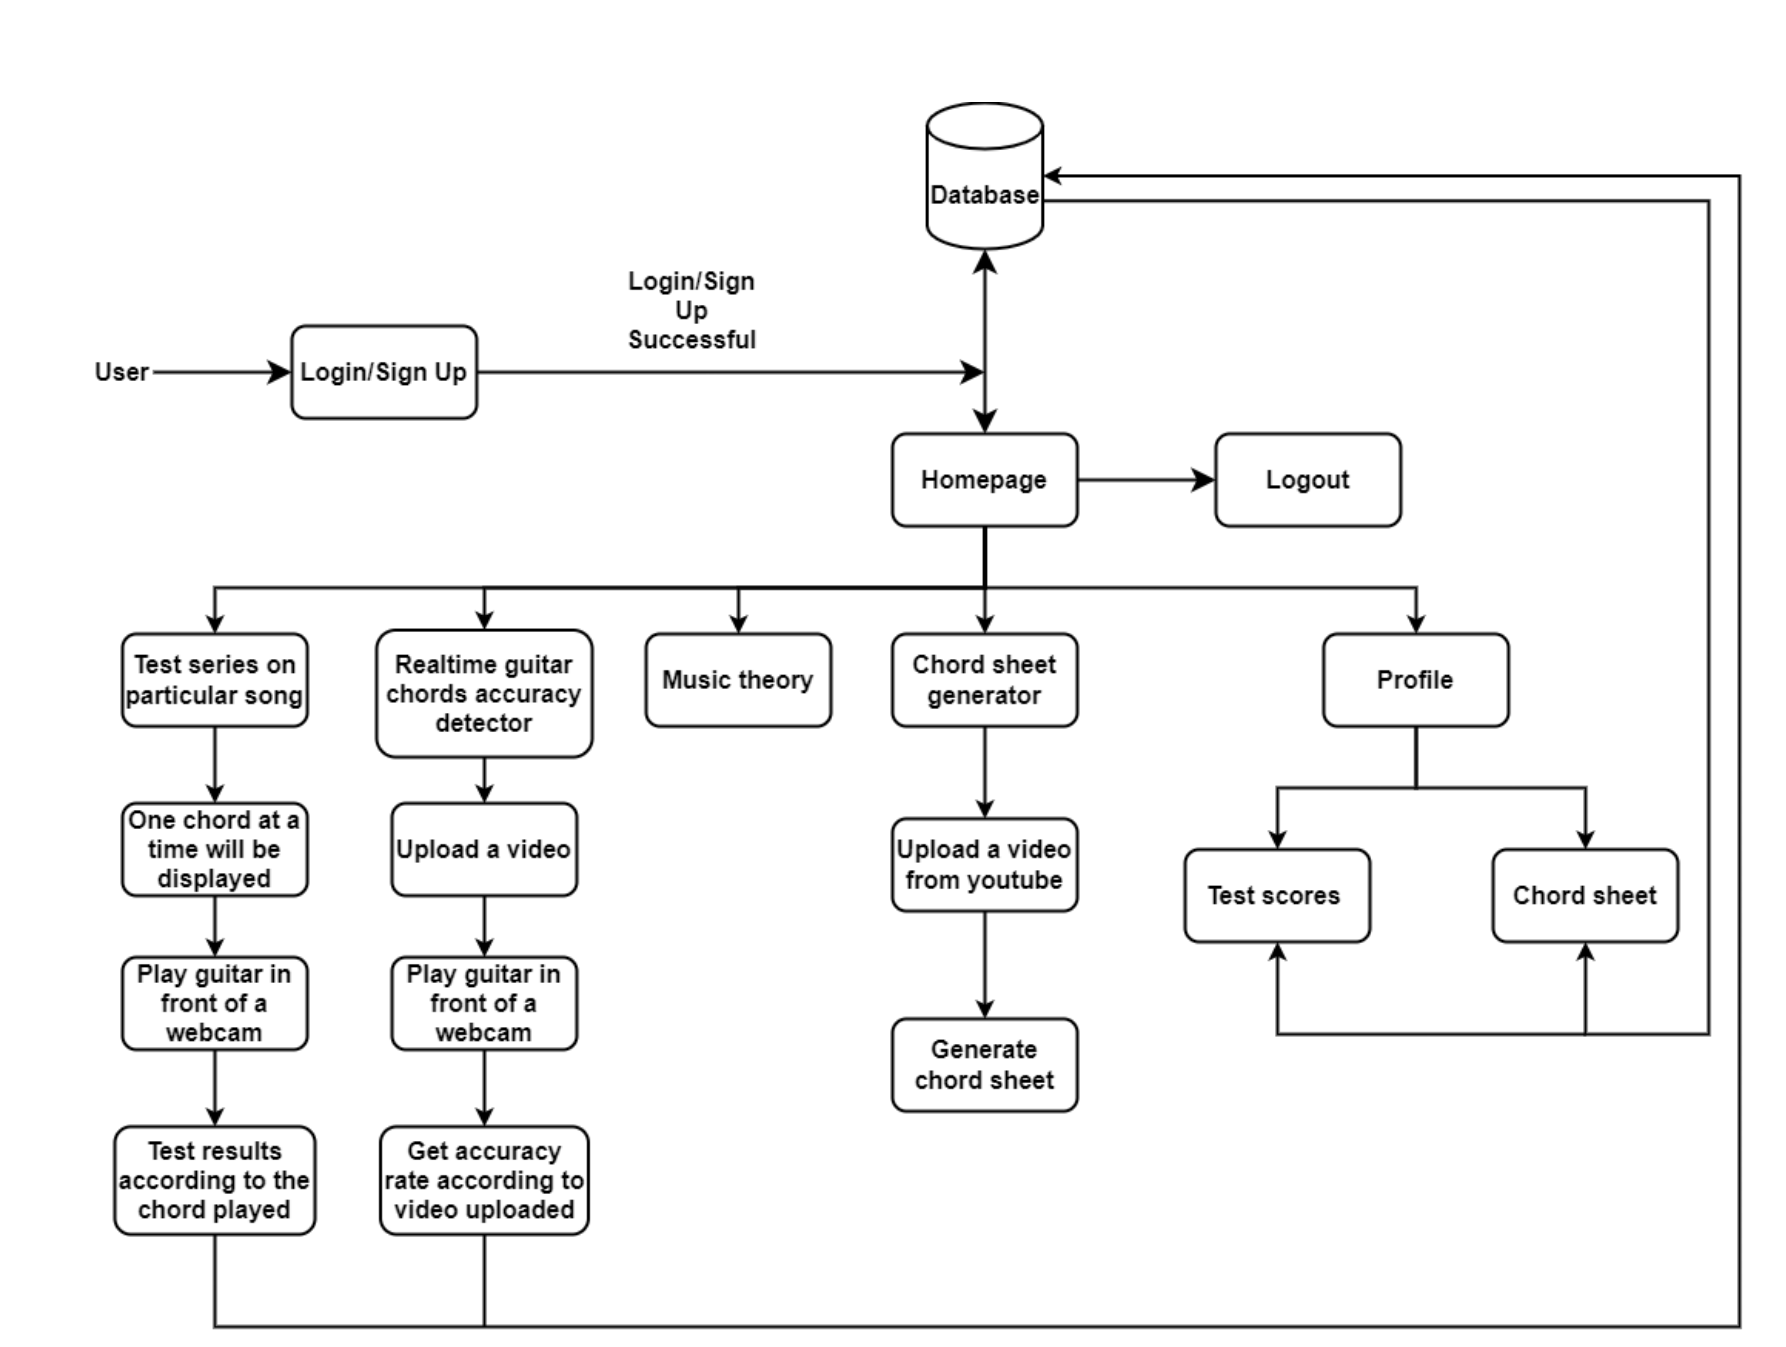
\includegraphics[width=\textwidth]{images/related-work/guitar-guru}
	\end{subfigure}
	\hfill
	\begin{subfigure}{0.39\textwidth}
		\centering
		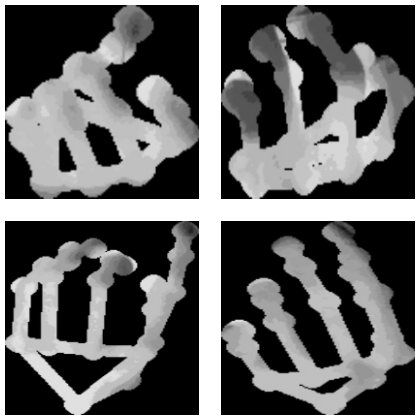
\includegraphics[width=\textwidth]{images/related-work/guitar-guru-chords}
	\end{subfigure}
	\caption{Architecture scheme and 4 chords (A, C, F, G) recognised from~\protect\cite{guitar-guru}}
	\label{fig:guitar-guru}
\end{figure}

Another trainer for pianists can be found in VRmonic~\cite{vrmonic-piano-trainer}, an immersive VR-based piano trainer
that uses the Unity Game Engine and a VR headset with a hand detector to compare the user's hand movements to the ones
of a virtual expert oracle, on a set of 48 scales for each of the 12 notes.
The goal of this project is not only to teach how to play the piano, but also how to play it with the
correct hand form, preventing long-term injuries in musicians of all levels.

The oracle's hand poses are recorded using a capture environment
in which some expert pianists perform the scales on an 88-key piano.
The pianist's hands are captured using a Microsoft Azure RGB-D camera mounted 88.25 cm above the piano.
Five trials are performed for each scale and the resulting joint positions are merged together into the final oracle positions by averaging the positions in each trial.

When running a training session, the user needs any VR headset that supports Unity and is capable of doing hand detection.
After having selected the note, scale, and beats per minute, the user can start to record a playback or run a playback by the oracle.
Pieces recorded by the user can be later played back together with the ones played by the expert oracle, creating an overlay of two pairs of hands, one belonging to the user and one to the oracle.
The user can set the tolerance level, which represents the number of collisions between corresponding joints on the two pairs of hands, to control the level of feedback on alignment with the expert.
VRmonic currently does not support real-time feedback.

VRmonic is a promising project with great potential.
Future development possibilities include adding support for real-time feedback mode,
the incorporation of qualitative feedback via large language models (LLM) to provide personalised voice-based
feedback based on the magnitude of the error, and the addition of further control over the pianist's posture
as well as the position of his hands.

\begin{figure}[ht]
	\centering
	\begin{subfigure}{0.55\textwidth}
		\centering
		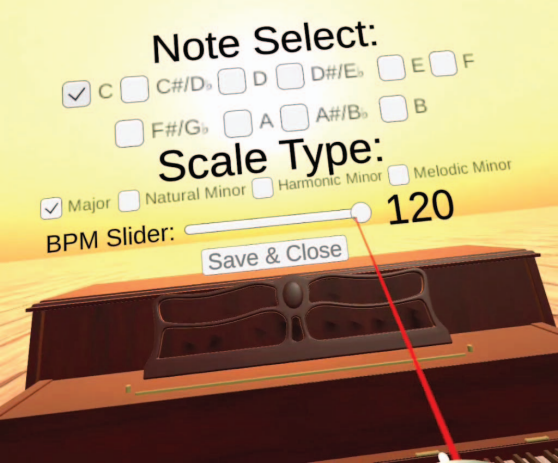
\includegraphics[width=\textwidth]{images/related-work/vrmonic}
	\end{subfigure}
	\hfill
	\begin{subfigure}{0.43\textwidth}
		\centering
		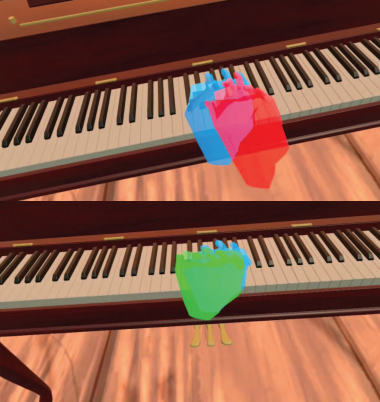
\includegraphics[width=\textwidth]{images/related-work/vrmonic-example}
	\end{subfigure}
	\caption{VRmonic interface and overlapping hands example: inaccurate vs accurate}
	\label{fig:vrmonic}
\end{figure}



	\chapter{System architecture}\label{ch:system-architecture}

In this chapter, the project is presented in its entirety, starting from the initial idea with the first prototype,
going through the various iterations, the choices made and the hypotheses discarded, up to the current,
but not final, version of the Keyrtual application.

\section{History of the project}\label{sec:history-of-the-project}
This project originally began in January 2023 as work for a paper~\cite{keyrtual} presented at the 20th International
Conference on Computer Analysis of Images and Patterns (CAIP 2023).
While the paper's version and the current version of the project are similar in purpose, they are completely different in implementation.
The main difference between the two is that the first one was not intended for mobile devices, but was essentially
a prototype designed to assess the general feasibility of the project,
although it was still meant to be suitable for low-end (non-mobile) devices.

In this first prototype, the procedure to use the program is longer and more cumbersome, and is summarized
in~\autoref{fig:keyrtual-leap-motion-method}.

\begin{figure}
	\center
	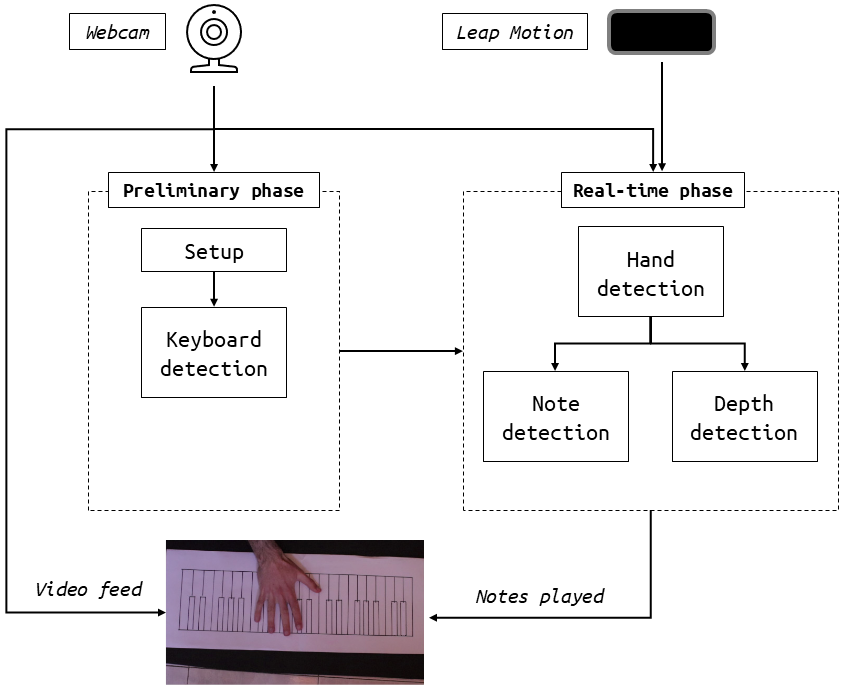
\includegraphics[width=0.8\textwidth]{first-prototype-architecture}
	\caption{Architecture of the first prototype}
	\label{fig:keyrtual-leap-motion-method}
\end{figure}

\subsection{Constraints}\label{subsec:constraints-prototype}

\paragraph{General constraints}
The paper sheet where the keyboard is drawn should have a sufficiently strong
contrast to the table, and the same applies to the keys drawn to the paper.

The camera and Leap Motion should also be placed at an adeguate distance
to be able to frame the paper and hands in their entirety.
They should be placed perpendicular to the table, so that they have as good a view as possible from above,
and oriented so that the user appears at the top.

\paragraph{Hardware prerequisites}
First, the use of an external webcam and a Leap Motion Controller is required.
These two devices should be placed next to each other perpendicular to the table on which the user intends to
use the drawn keyboard, so as to have an elevated view of the keyboard and the user's hands.

As for the computer, there is no special prerequisite since the program is designed to
be used even on low-end devices.

\subsection{Preliminary phase}\label{subsec:preliminary-phase-prototype}
The preliminary phase is divided into two parts: the background subtraction part and the keyboard detection part.
The whole process is illustrated in~\autoref{fig:preprocessing-prototype}

\paragraph{Background subtraction}
Once the components are assembled, we move on to the preliminary stage of keyboard detection.
For this purpose, a background subtraction operation is first performed, which consists of taking two pictures:
the first will be a picture of the table without the keyboard, while the second will include the keyboard.
By calculating the differences between the two images, the background is removed, leaving only the keyboard.

\paragraph{Keyboard detection}
Once the area of the image on which the keyboard is located has been identified, we proceed with key detection.
This is done by applying different filters to the image to increase the contrast between white sheet and black keys,
and using classic algorithms such as Canny edge detector, probabilistic Hough Transform procedure
and K-means clustering to extrapolate the rows that make up the keyboard keys.
These rows are separated according to their length and position to separately identify white keys and black keys.

\begin{figure}[t]
	\centering
	\begin{subfigure}{0.32\textwidth}
		\centering
		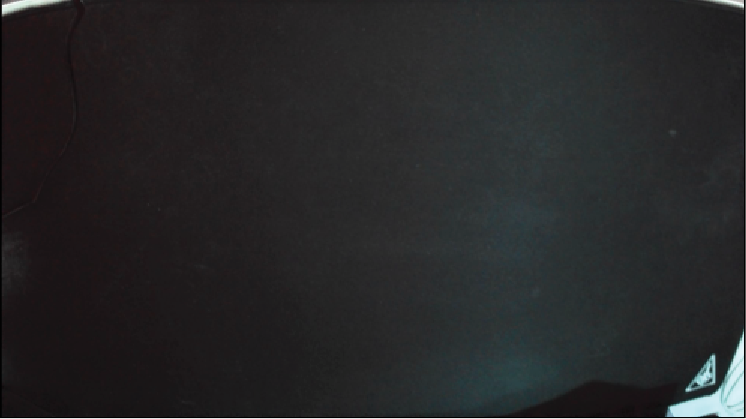
\includegraphics[width=\textwidth]{prototype-method/setup-1}
		\caption{}
		\label{fig:setup_background}
	\end{subfigure}
	\hfill
	\begin{subfigure}{0.32\textwidth}
		\centering
		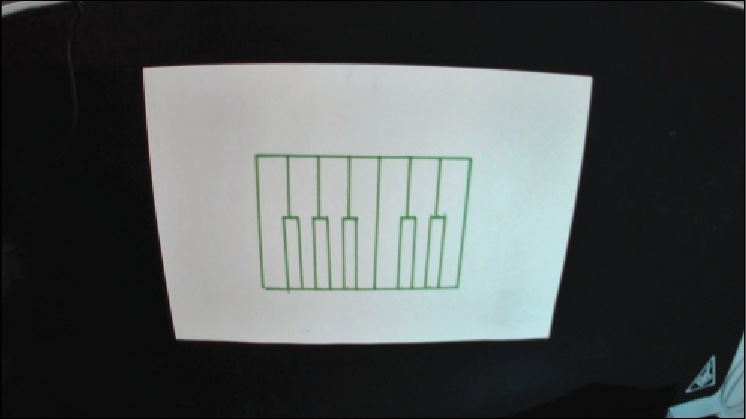
\includegraphics[width=\textwidth]{prototype-method/setup-2}
		\caption{}
		\label{fig:setup_keyboard}
	\end{subfigure}
	\hfill
	\begin{subfigure}{0.32\textwidth}
		\centering
		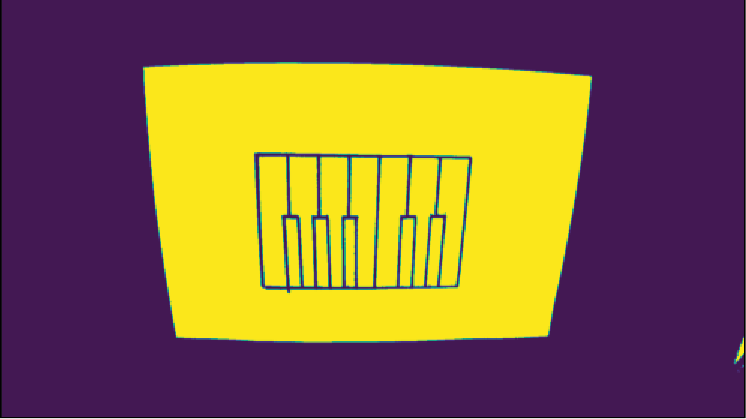
\includegraphics[width=\textwidth]{prototype-method/background}
		\caption{}
		\label{fig:keyboard_background}
	\end{subfigure}
	\hfill
	\begin{subfigure}{0.32\textwidth}
		\centering
		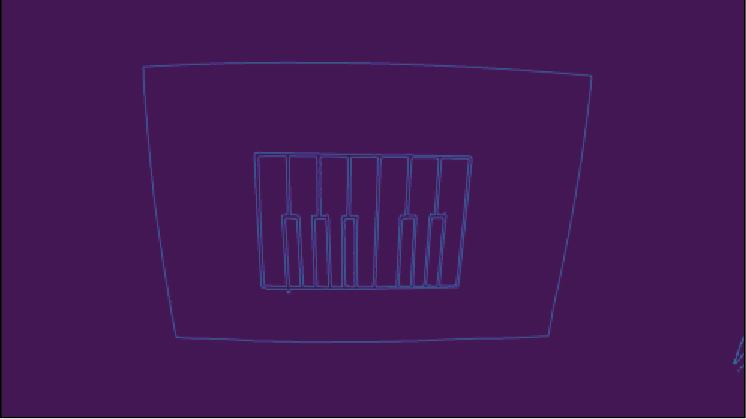
\includegraphics[width=\textwidth]{prototype-method/edges}
		\caption{}
		\label{fig:canny-prototype}
	\end{subfigure}
	\hfill
	\begin{subfigure}{0.32\textwidth}
		\centering
		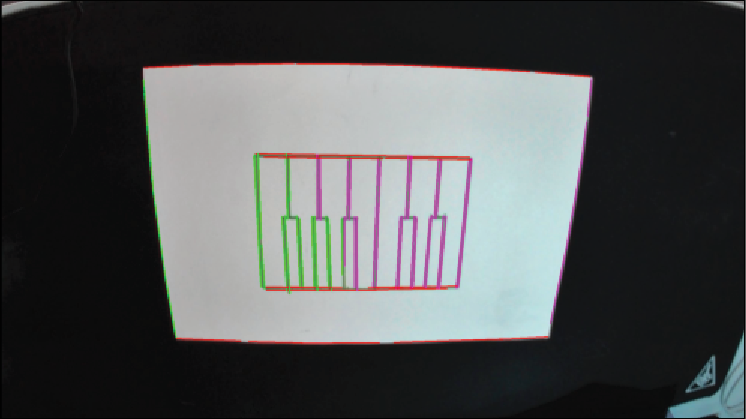
\includegraphics[width=\textwidth]{prototype-method/lines}
		\caption{}
		\label{fig:hough}
	\end{subfigure}
	\hfill
	\begin{subfigure}{0.32\textwidth}
		\centering
		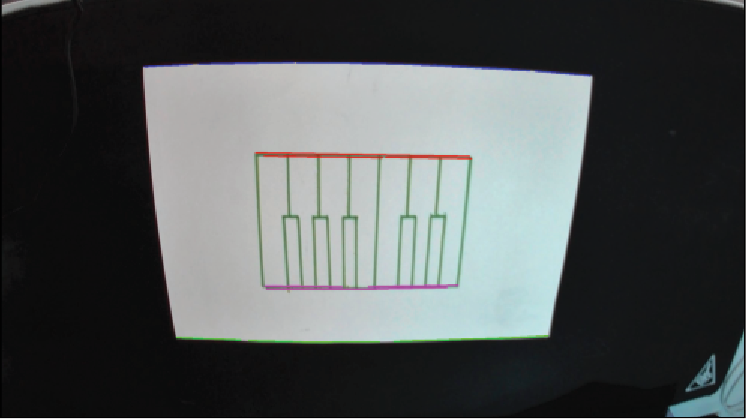
\includegraphics[width=\textwidth]{prototype-method/hor-lines}
		\caption{}
		\label{fig:hor_lines}
	\end{subfigure}
	\hfill
	\begin{subfigure}{0.32\textwidth}
		\centering
		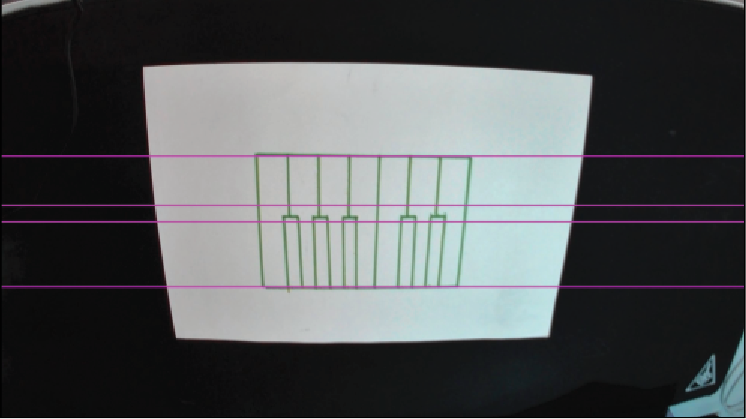
\includegraphics[width=\textwidth]{prototype-method/borders}
		\caption{}
		\label{fig:borders}
	\end{subfigure}
	\hfill
	\begin{subfigure}{0.32\textwidth}
		\centering
		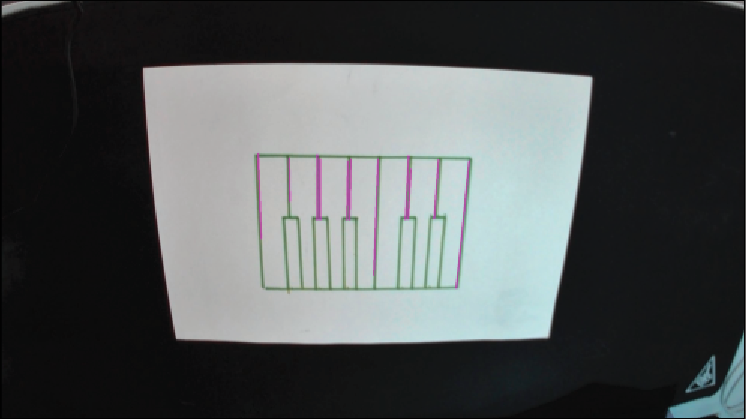
\includegraphics[width=\textwidth]{prototype-method/white-tiles}
		\caption{}
		\label{fig:white_tiles}
	\end{subfigure}
	\hfill
	\begin{subfigure}{0.32\textwidth}
		\centering
		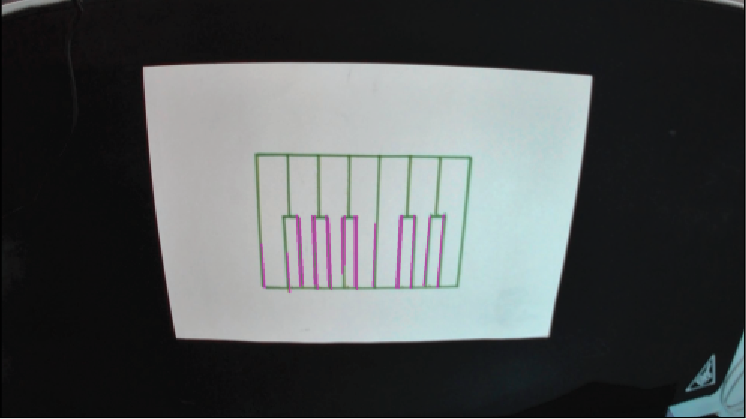
\includegraphics[width=\textwidth]{prototype-method/black-tiles}
		\caption{}
		\label{fig:black_tiles}
	\end{subfigure}
	\caption{
		Preliminary phase pipeline.
		(a) First frame;
		(b) Second frame;
		(c) Background highlight;
		(d) Canny edge detection;
		(e) Hough transformation;
		(f) Horizontal lines detection;
		(g) Borders highlight;
		(h) White tiles highlight;
		(i) Black tiles highlight.
	}
	\label{fig:preprocessing-prototype}
\end{figure}

\subsection{Real-time phase}\label{subsec:real-time-phase-prototype}
After the setup is finished, we move on to the real-time phase: the user can now play on the
keyboard, and the program will play back the notes played.
In this phase, MediaPipe and the Leap Motion Controller are used in conjunction to detect which key is being pressed
and if it is actually pressed, respectively.

This is necessary because MediaPipe, despite its accuracy in detecting the 2D position of the hands on the image,
is not at all accurate in detecting the third coordinate, that is, the distance of the fingers from the camera.

\paragraph{Sensor fusion}
For this, a sensor fusion technique is used between MediaPipe and the Leap Motion Controller: MediaPipe is
constantly used to detect the presence and position of hands on the screen, but it is the Leap Motion
Controller that triggers the process of playing a sound: when the controller detects that a finger has fallen
below a certain threshold, it uses the coordinates provided by MediaPipe to determine the button on which the
lowered finger is located, and the corresponding note is played using the MIDI protocol\@.


\section{Evaluation of Porting Strategies}\label{sec:evaluation-of-porting-strategies}
Following the prototype publication, various intermediate solutions were hypothesised, tested and discarded
before arriving at the current version of the Keyrtual mobile application.
This section will explore the various steps that led us to the final version,
the unsuccessful attempts and the reasons why certain choices were made.

\subsection{Depth vision}\label{subsec:depth-vision}
Nowadays, the presence of two or more photo sensors has become the standard for all smartphones, even low-end ones.
Among the sensors that can be found on smartphones there are for example
depth sensors, macro sensors, wide-angle sensors and tele sensors.

One of the first ideas, when we started thinking about porting the project to smartphones,
was to use these different sensors to derive information about the position of the hands
in the three-dimensional space of the scene, in two possible ways:
\begin{itemize}
	\item \textit{Depth sensor:} directly use the smartphone's depth sensor to obtain depth information on the
	playing fingers, to be combined with the information obtained from the RGB sensor and MediaPipe,
	just like in the first prototype.
	\item \textit{Stereo vision:} use two different camera sensors at the same time to capture two images
	of the same scene, from two slightly different points of view, and then use classic stereo
	vision algorithms to derive the depth of the hands in the scene.
\end{itemize}

At first glance, both of these methods might seem excellent for solving the problem of depth
ambiguity in single-perspective images, but unfortunately both have technical
difficulties that make them practically unusable in our use case.

\subsubsection{Depth sensor}
The depth sensor in smartphones is used, among other things, to improve focus, sharpness and to apply visual
effects on the final image, such as background blur and focus on an object in the foreground.
The idea of using this sensor to derive depth information on the hand is unfortunately
unrealistic given the low resolution and sensitivity of this type of sensor.

In our case, we need an accuracy in detecting depth in the order of a centimetre.
In fact, to detect the touch of a finger, we need to detect a small change in depth, of about 1 cm,
in the area of a single finger, about 1 cm$^2$ in size, at a distance from the sensor of about 40 cm.

This accuracy could perhaps be achieved by the sensors built in a handful of high-end smartphones, but since
one of the goals of this project is to reach as many devices as possible, this method was abandoned very early on.

\subsubsection{Stereo vision}
This method presents even greater technical difficulties than the previous one.
Firstly, as mentioned above, although smartphones are equipped with multiple camera sensors,
they all perform a different function and differ deeply in terms of size, accuracy and the type of output produced.
To use the stereo vision technique, one would need a smartphone with two identical cameras.

Moreover, the presence and positioning of these sensors on the back of the smartphone is by no means regular,
and can vary greatly from model to model.
This would be a major obstacle in using stereo vision algorithms,
which depend on the position and proximity of the sensors used.

\begin{figure}[ht]
	\captionsetup[subfigure]{labelformat=empty}
	\centering
	\begin{subfigure}{0.3\textwidth}
		\centering
		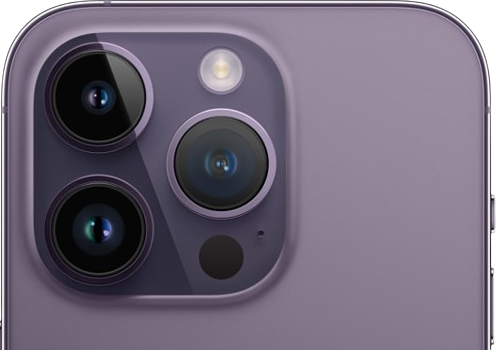
\includegraphics[width=\textwidth]{images/back-camera-iphone-14-pro}
		\caption{Iphone 14 Pro}
	\end{subfigure}
	\hfill
	\begin{subfigure}{0.3\textwidth}
		\centering
		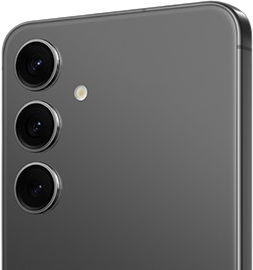
\includegraphics[width=\textwidth]{images/back-camera-galaxy-s24}
		\caption{Samsung Galaxy S24}
	\end{subfigure}
	\hfill
	\begin{subfigure}{0.3\textwidth}
		\centering
		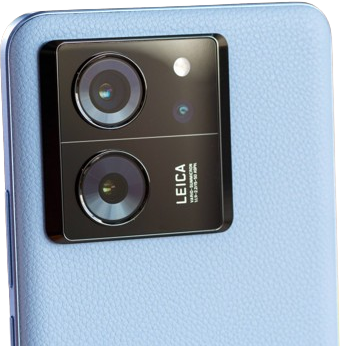
\includegraphics[width=\textwidth]{images/back-camera-redmi-13t}
		\caption{Xiaomi 13T}
	\end{subfigure}
	\caption{Different models of smartphone with different camera sensor number and position.}
	\label{fig:back-cameras}
\end{figure}

\subsubsection{Dedicated software}
We also considered the possibility of using dedicated software to calculate a depth map from an RGB image,
such as MiDaS~\cite{midas}.
Unfortunately, these models are not designed for use on mobile devices,
and require computing power that is not available on smartphones.

Although there are versions designed specifically for mobile devices,
the resulting depth maps are not precise enough for our purpose.

\subsection{MediaPipe for 3D coordinates}\label{subsec:mp-for-3d}
MediaPipe's hand detection feature not only detects hand landmarks as 2D coordinates in the image,
but also produces extra coordinates representing the position of the landmarks in 2.5D space.
In the 2.5D space, in addition to the existing $x$ and $y$ axes, a new $z$ axis is added to represent the landmark
depth with the depth at the wrist being the origin, and the smaller the value the closer the landmark is to the camera.

Among the methods hypothesised for porting the project to smartphones was to use this new coordinate to assess
whether a finger was pressing on a button, using the $z$ axis value.
This method immediately revealed a number of problems, including the fact that the $z$ coordinate,
being derived from a single RGB image, is not precise and is also very flickering.

In addition, the $z$ coordinate is not expressed in absolute reference but in reference to the landmark located in
the wrist, which makes its value variable not only according to the position of the individual landmark
but according to the position of the entire hand in relation to the wrist.

\subsection{Point of view}\label{subsec:pov}
A very important difference between the new and the old prototype is the change in the positioning of the camera.
In the first prototype we chose to use a 90\degree \ angle, which gave us a very good view of the keyboard,
precise information on the position of the hands on the plane in relation to the keys and, thanks
to the Leap Motion sensor, precise information on the distance and position of the hands in three-dimensional space.
This results in complete information on the $x_w$ and $y_w$ axes ($x$ and $y$ world axes) given by the RGB sensor,
and excellent information on the $z_w$ axis given by the Leap Motion sensor.

In the new version, in which we only have the RGB sensor, using the same positioning of the camera,
the $z_w$ axis information is totally lost.
This can be partially recovered thanks to MediaPipe, which however does not provide sufficiently precise
depth coordinates but rather inconsistent and flickering, so we could not rely solely on them.

Instead, we preferred to exploit a 45\degree \ angle of the camera in order to make the best use of the partial
information this viewpoint provides us with regarding the $z_w$ axis.
Changing the angle from 90\degree \ to 45\degree, in fact,
provides us with partial information on the $z_w$ axis that is completely absent in the top view.
The two methods are illustrated in \autoref{fig:camera-povs}.

The first method, that of the old prototype explained
in~\autoref{subsec:real-time-phase-prototype}~\nameref{subsec:real-time-phase-prototype},
gave complete information on the $x_w$ and $y_w$ axes, but no information on the $z_w$ axis.
This shortcoming, shown in \autoref{fig:camera-pov-90}, was compensated for by the use of the Leap Motion sensor,
which provided accurate depth data and allowed the system to function correctly.

However, this method is no longer usable now that we only have an RGB camera at our disposal,
and we were therefore forced to change to a different angle.
This new viewpoint has the advantage of gaining partial information about the $z_w$ axis, at the cost of a partial
loss of information about the $y_w$ axis, both of which are visible in \autoref{fig:camera-pov-45}.

The result is that the $y_w$ and $z_w$ axes are partially merged and ``compressed'', becoming part of the same
$y_s$ axis ($y$ screen axis, given by MediaPipe), while the $x_w$ axis
maintains a virtually exact correspondence with the $x_s$ axis.

\begin{figure}[ht]
	\centering
	\begin{subfigure}{0.49\textwidth}
		\centering
		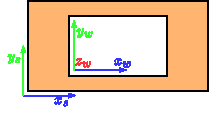
\includegraphics[width=\textwidth]{images/application/camera-pov-90}
		\caption{Camera angle at 90\degree}
		\label{fig:camera-pov-90}
	\end{subfigure}
	\hfill
	\begin{subfigure}{0.49\textwidth}
		\centering
		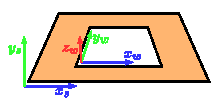
\includegraphics[width=\textwidth]{images/application/camera-pov-45}
		\caption{Camera angle at 45\degree}
		\label{fig:camera-pov-45}
	\end{subfigure}
	\caption{
		Different points of view of the camera on the paper sheet.
		The lower the angle, the more precision about axis $z_w$ but less precision about $y_w$.
	}
	\label{fig:camera-povs}
\end{figure}

The partial loss of information on the $y_w$ axis, however, is not a problem at all: it is in fact only used for
note recognition, and this only occurs when a touch is recognised, i.e.\ when the finger presses directly on the paper.
The loss of information on the $y_w$ axis, therefore, does not affect note recognition at all,
nor the functioning of the application in general.

Thanks to the presence of the frame area, during keyboard detection,
we can force the correct positioning of the smartphone, guaranteeing the success of real-time phase.


\section{Unity}\label{sec:unity}
Unity is a professional, robust and versatile game development platform
that has gained widespread popularity~\cite{unity-technical-survey} for its ability to create both 2D and 3D applications.
The Unity editor is cross-platform, being supported on Windows, macOS and Linux, and its engine supports builds
for more than 19 different platforms, including mobile and desktop devices, consoles and VR devices.

Developed by Unity Technologies, it has evolved into a powerful tool for implementing
high performance applications~\cite{unity-interview-high-speed}, used by developers worldwide for a variety of projects,
ranging from games to simulations, augmented reality~\cite{marco-ar, marco-ar-mano},
and virtual reality~\cite{marco-vr} applications.

Augmented reality applications made with Unity can easily be used in a
classroom~\cite{ar-application-in-classroom-taxonomy, ar-for-preschool-children, vr-and-ar-for-learning, educational-ar}
as an innovative and interactive teaching method for children, with examples of its usage in the teaching of subjects such as
Astronomy~\cite{ar-astronomy}, Volcanology~\cite{ar-volcanology}, Engineering~\cite{ar-engineering},
Medicine~\cite{ar-medicine} and more~\cite{ar-microeconomics, ar-animals}.
This makes Unity the perfect tool for our project.

Our application requires the use of the OpenCV and MediaPipe libraries, and is written entirely in \texttt{C\#} within the Unity Engine.
This led us to the adoption of the corresponding plugins within the game engine.
The exact versions of Unity and plugins used within the project are:
\begin{itemize}
	\item Unity Editor: 2022.3.18f1
	\item OpenCV for Unity: 2.5.8
	\item MediaPipe for Unity: 0.14.1
\end{itemize}

\subsection{OpenCV}\label{subsec:opencv-for-unity}
OpenCV for Unity is a very popular plugin for using OpenCV within the Unity development environment.
It can be purchased from the Unity Asset Store and easily imported into a project.
From there, its use differs little from what it would be in \texttt{C++} or \texttt{Python}:
it supports practically all the functions and constants present in the original module,
while maintaining an API identical to its \texttt{C++} counterpart.

The support for WebCamTexture makes OpenCV for Unity easy to use in applications that need to perform real-time image processing,
which makes it an excellent choice for our project.

\subsection{MediaPipe}\label{subsec:mediapipe-for-unity}
MediaPipe for Unity is a native plugin which ports the \texttt{C++} MediaPipe API to \texttt{C\#}, one by one,
so that it can easily be used within the Unity development environment.
It can be installed from the documentation page and be directly imported into the project.
Thanks to the precise documentation, the various example scenes and the clear and comprehensive tutorial,
using MediaPipe in Unity is quick and easy.

This library supports all major desktop operating systems (Linux, macOS and Windows) as well as the mobile systems
Android and iOS, for which GPU mode can also be enabled, which is why we chose to use this library in our project.


\section{Method}\label{sec:method}
As of now, the project has made progress towards user-friendliness and accuracy, and all that is needed
is a smartphone with the application installed and a paper sheet.
The pipeline is still divided into a preliminary phase and a real-time phase,
but now all the work is done by a single device instead of three different devices.

Launching the application immediately gives visual feedback from the camera on the smartphone screen:
the user directly sees what they are framing with the camera, making the preliminary phase much faster and easier,
also thanks to a visual guide in transparency on the image, which is used to aim at the keyboard.

Once the keyboard is centered in the visual guide, the user can press a button on the application interface
to start the process of detecting the keyboard.
The detection process takes less than a second, and once it is finished, the screen will display in transparency the
keys detected by the application, so that the user can assess whether the process was successful and,
if they are not satisfied, repeat it as many times as necessary.

Both the visual guide and the keys in transparency can be hidden either before or after the preliminary step.
When the user is satisfied with the result of the preliminary stage, they can immediately start playing on the
semi-virtual keyboard, without any other interaction with the application.

The entire process is shown in~\autoref{fig:keyrtual-smartphone-method}
and the implementation details are explained in the following paragraphs.

\begin{figure}[ht]
	\centering
	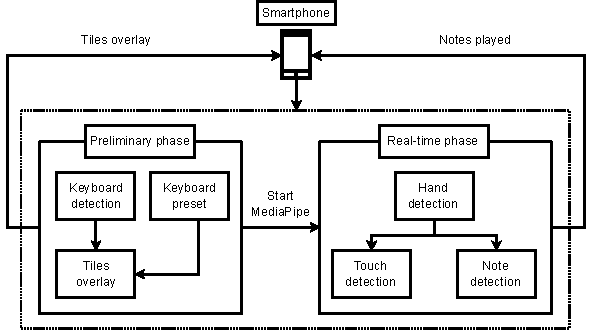
\includegraphics[width=0.8\textwidth]{images/application/architecture}
	\caption{Architecture of the current version}
	\label{fig:keyrtual-smartphone-method}
\end{figure}

\subsection{Constraints}\label{subsec:constraints}

\paragraph{General constraints}
The sheet should be a common white A4 sheet and the keyboard should be drawn in black or blue for better contrast.
There are no constraints on the contrast between the paper sheet and table due to the new background subtraction method.

The phone should be placed at a sufficient distance to frame the paper and hands in their entirety (experimentally
we have found that about 40 cm is fine) in a way such that the user, relative to the camera, appears to be on the top side
of the image and the paper on the bottom side of the image.

\paragraph{Hardware prerequisites}
No special prerequisites are required to run the application.
Thanks to the possibility of increasing and decreasing the FPS with which to run MediaPipe,
which is the most computationally demanding component,
it is possible to sacrifice some response speed to ensure that the application works on low-end phones.

\subsection{Preliminary phase}\label{subsec:preliminary-phase}
The preliminary phase still consists of background subtraction and keyboard detection, but the process to follow is much
faster, intuitive and automated.

All the single steps of this phase are shown in~\autoref{fig:preprocessing}.

\paragraph{Image acquisition}
As soon as the application is opened, the user can immediately go to the preliminary step of keyboard detection.
Due to the high mobility of the smartphone and the immediate visual feedback from the screen,
no real background subtraction process is required during this phase: a perimeter is drawn on the smartphone screen
around the area within which the application expects the user to frame the drawn keyboard.

When the user frames the keyboard in the perimeter and presses the button to start the detection process,
the application takes an image with a resolution of $1280 \times 720$, a reasonable resolution for all modern smartphones,
and cuts off from the image all the area outside the perimeter, keeping only the area where the keyboard is located.
This makes the background subtraction process much more effective and accurate,
and also much faster since no particular algorithm is used.

Since smartphone webcams, used via Unity, have an image correction and automatic focus function,
we had to take countermeasures to prevent the webcam from automatically
moving the focus outside our perimeter, making the detection phase inaccurate.
To do this, we forced the webcam's focus on the centre of the perimeter via Unity's API\@.

The perimeter and the result for this phase are shown in \autoref{fig:perimeter} and \autoref{fig:mat}.

\paragraph{Preprocessing}
Before performing the actual keyboard detection, we go through a second but very important preprocessing step:
filters are applied to the cropped keyboard image to highlight the 
keys drawn in black against the white background of the paper sheet.

The image is converted to grayscale and Canny edge detector algorithm is applied to highlight the black lines.
Two iterations of closing morphological operator are applied to the image, to enhance the visibility of the edges found by Canny.
We are not quite interested in cleaning those small white pixel spots that appear scattered over the image
because they will be removed during the next step.

The single steps of this phase can be seen in \autoref{fig:canny} and \autoref{fig:canny-closed}.

\paragraph{Tiles detection}
At this point, we proceed to the actual keyboard detection.
After extensive experimentation, we concluded that the old method using probabilistic Hough Transform to detect lines
was too inaccurate and inconsistent, and moreover wouldn't allow us to detect non-straight lines,
which is a fundamental prerequisite in this case since we would like to detect hand-drawn keyboards.
Therefore, we opted for a much simpler and more robust method: contour detection~\cite{contour-detection}.

The contour detection procedure is applied to edges obtained from the previous step.
The contours thus obtained, however, are filtered in several ways, eliminating:
\begin{itemize}
	\item contours with width greater than height (non-vertical)
	\item contours with area smaller than 300 pixels
	\item contours with area greater than 5\% of the image
\end{itemize}
The contours left represent the keys drawn on the paper and are shown in \autoref{fig:contours}.

\paragraph{Tiles overlay}
With the previously obtained contours, the overlay with the keys drawn in transparency is created and shown to the user.
To make the overlay look like a real keyboard, the keys are colored white or black according to their length:
longer keys are white and shorter keys are black.

The result can be seen in \autoref{fig:tiles-overlay}

\paragraph{Notes detection}\label{par:notes-detection}
The contours are sorted using the horizontal center as the sorting criteria.
An image is then created with the same size as the original, initially all black,
which is colored only inside the areas of the contours found.
The areas are colored with a gray scale starting at 1 and going up by 1 for each key.

The color for each key represents an index, starting from 1 up to the number of keys found,
which is used to determine the note number to be played according to the MIDI protocol.
The details of this method are explained in \autoref{subsubsec:notes-detection}~\nameref{subsubsec:notes-detection}.

The final result is shown in \autoref{fig:notes}.

\begin{figure}[ht]
	\centering
	\begin{subfigure}{0.49\textwidth}
		\centering
		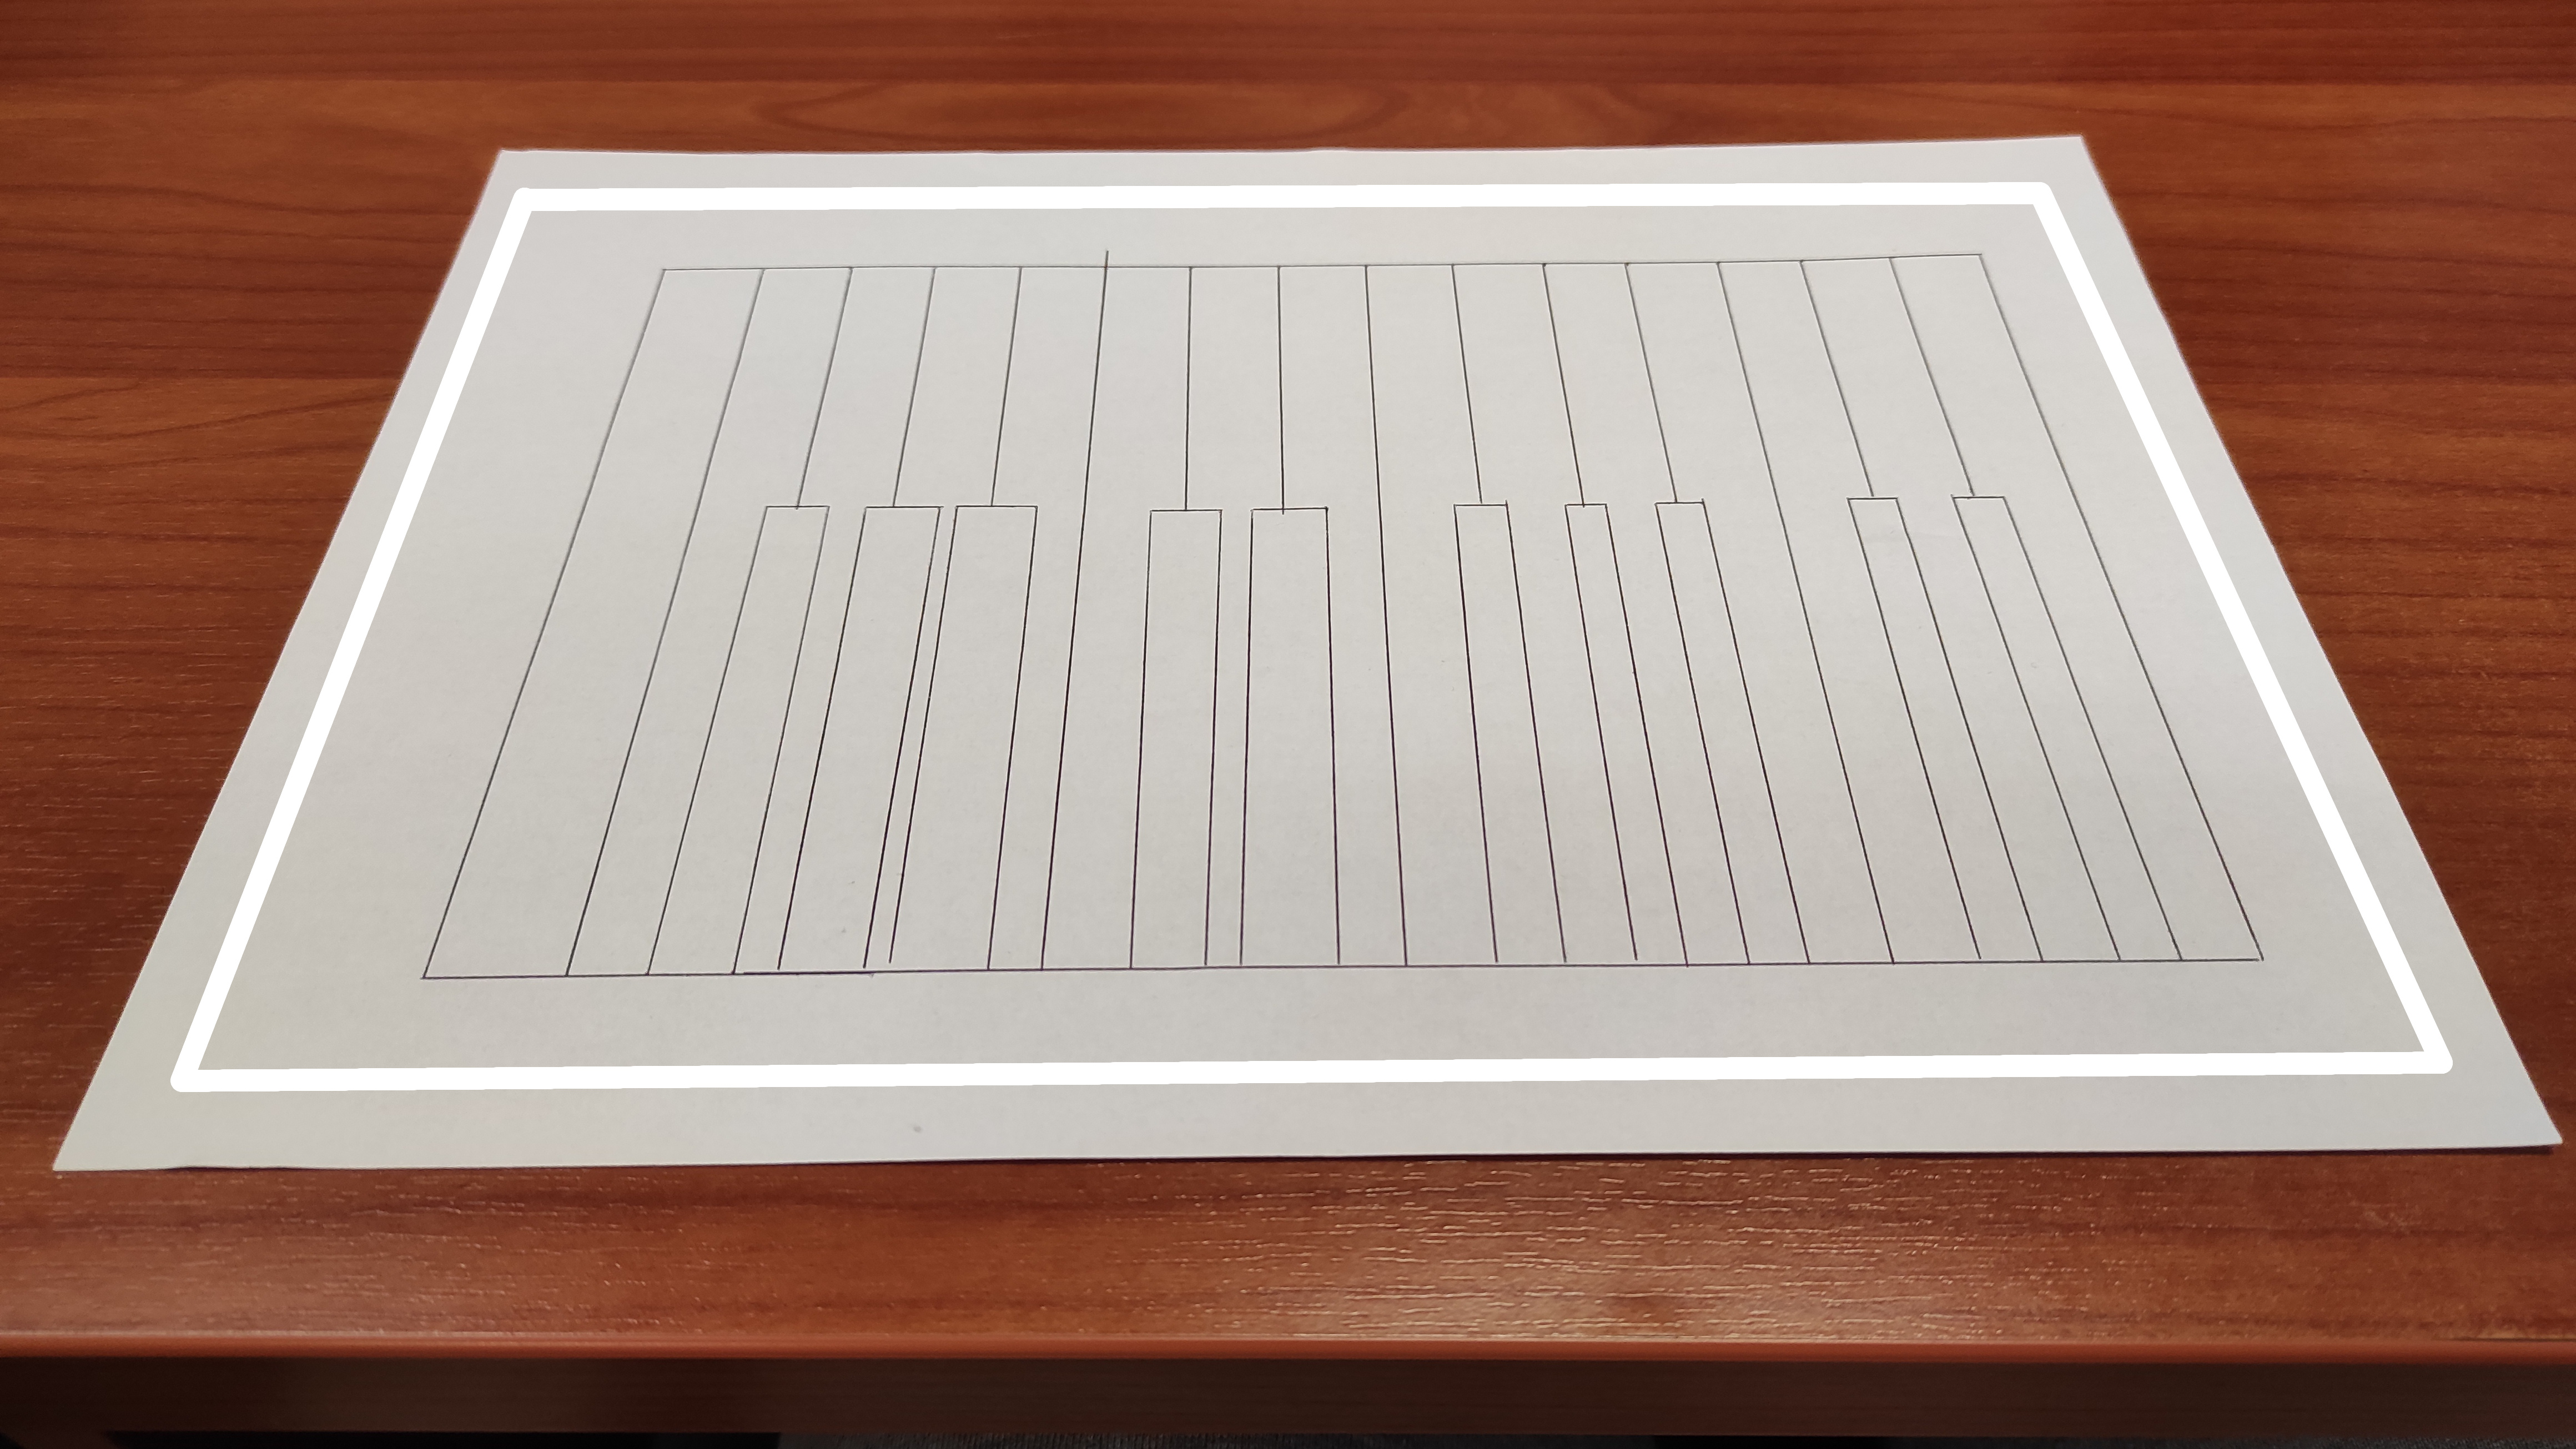
\includegraphics[width=\textwidth]{images/application/45deg/camera-with-frame}
		\caption{}
		\label{fig:perimeter}
	\end{subfigure}
	\hfill
	\begin{subfigure}{0.49\textwidth}
		\centering
		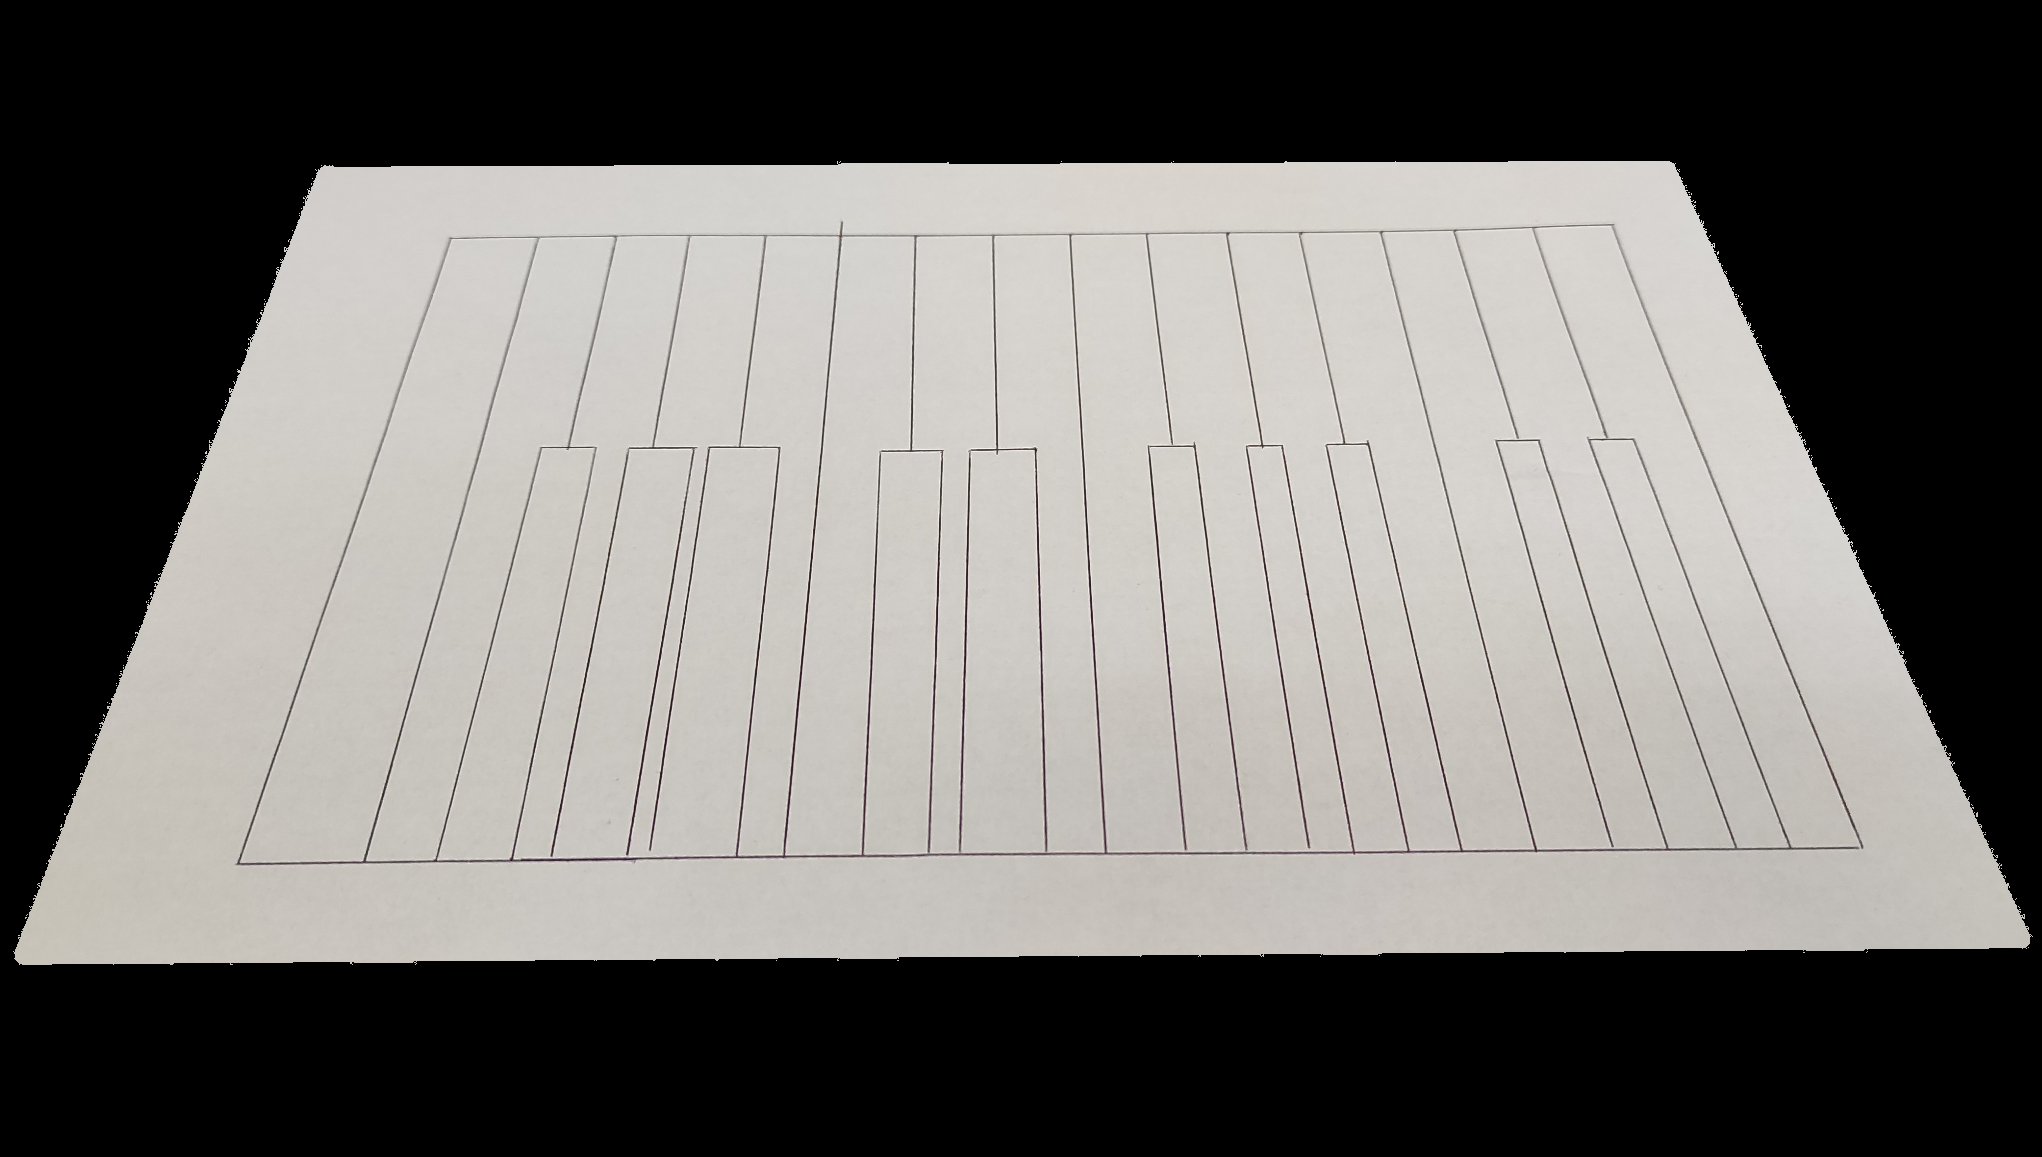
\includegraphics[width=\textwidth]{images/application/45deg/masked}
		\caption{}
		\label{fig:mat}
	\end{subfigure}
	\hfill
	\begin{subfigure}{0.49\textwidth}
		\centering
		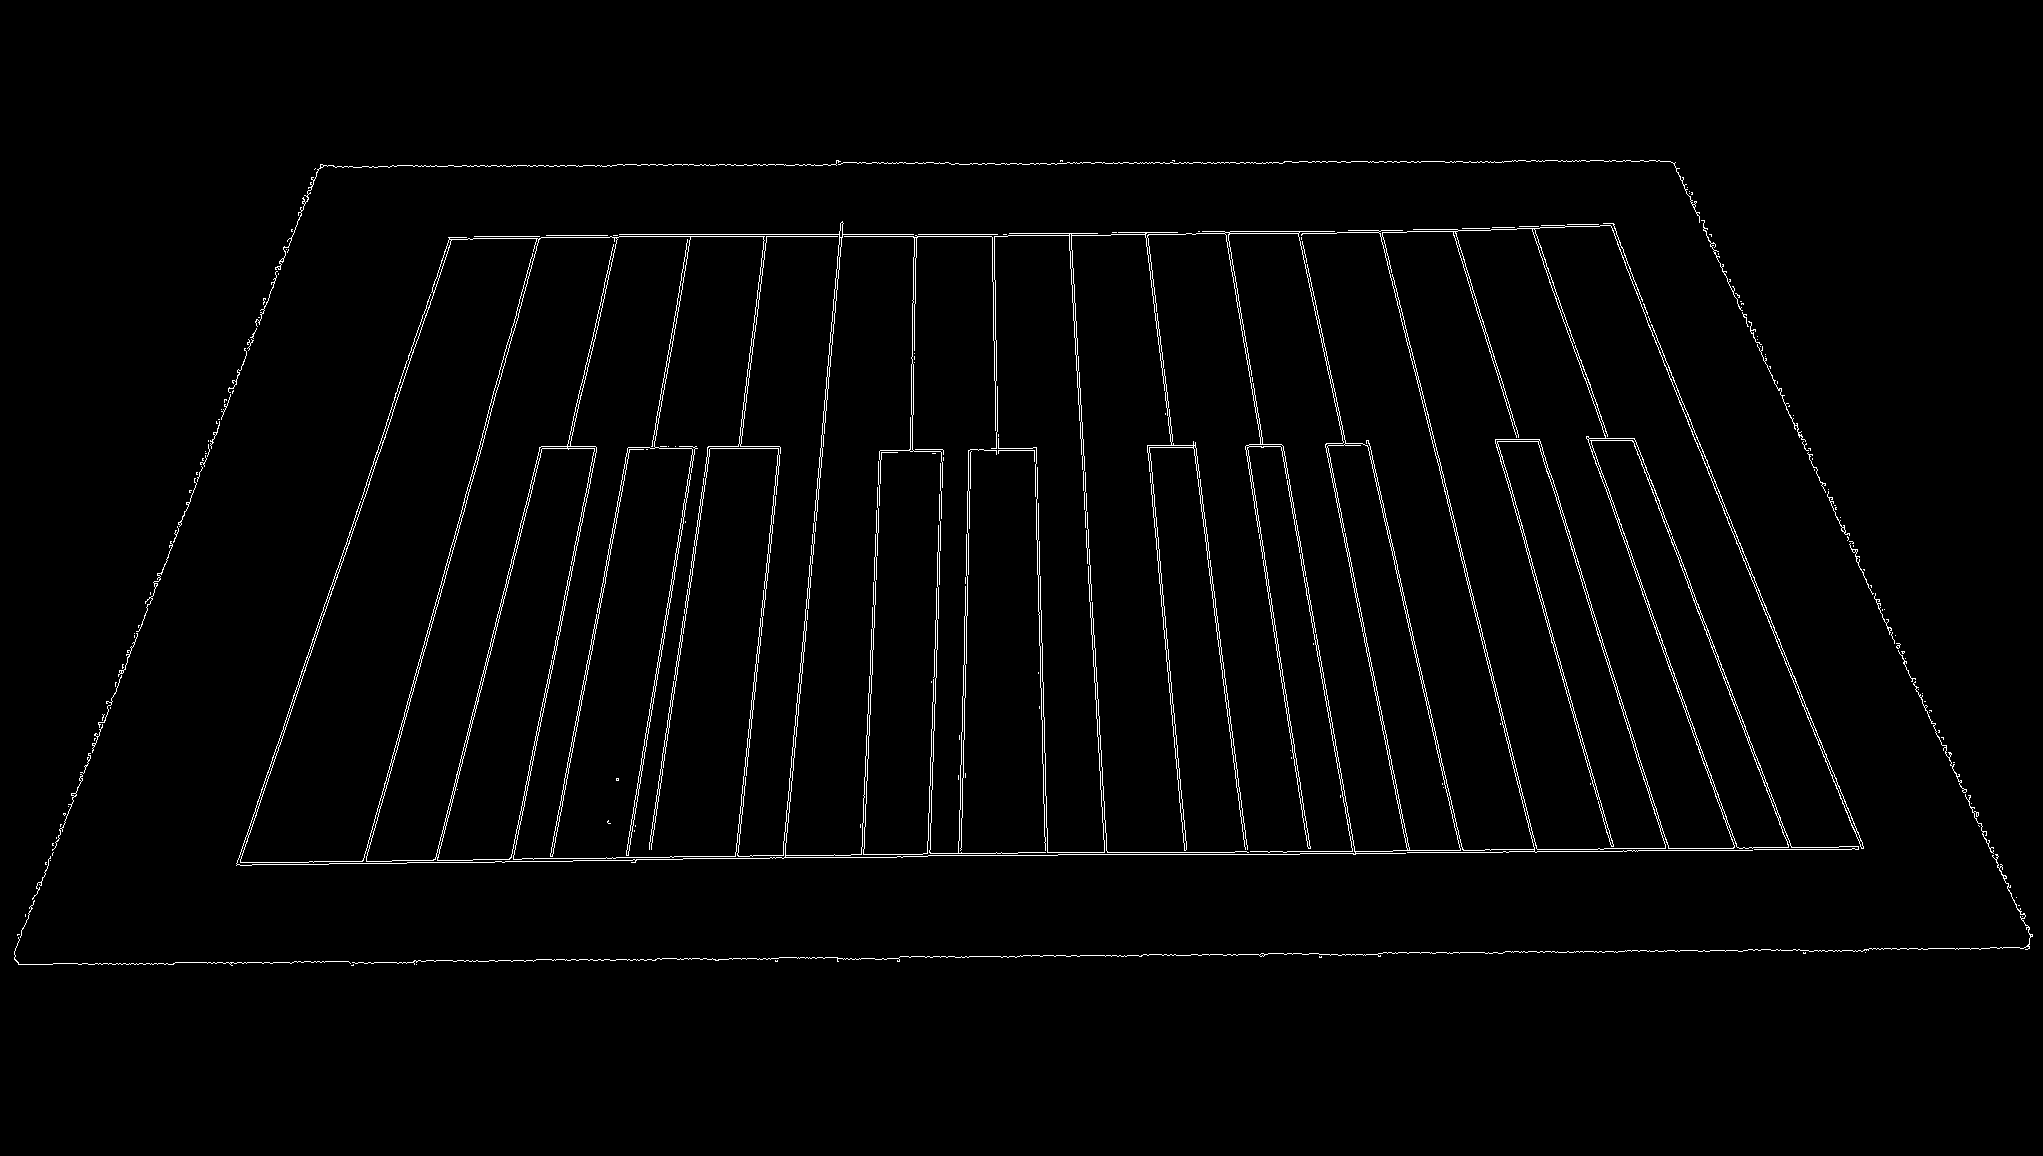
\includegraphics[width=\textwidth]{images/application/45deg/canny}
		\caption{}
		\label{fig:canny}
	\end{subfigure}
	\hfill
	\begin{subfigure}{0.49\textwidth}
		\centering
		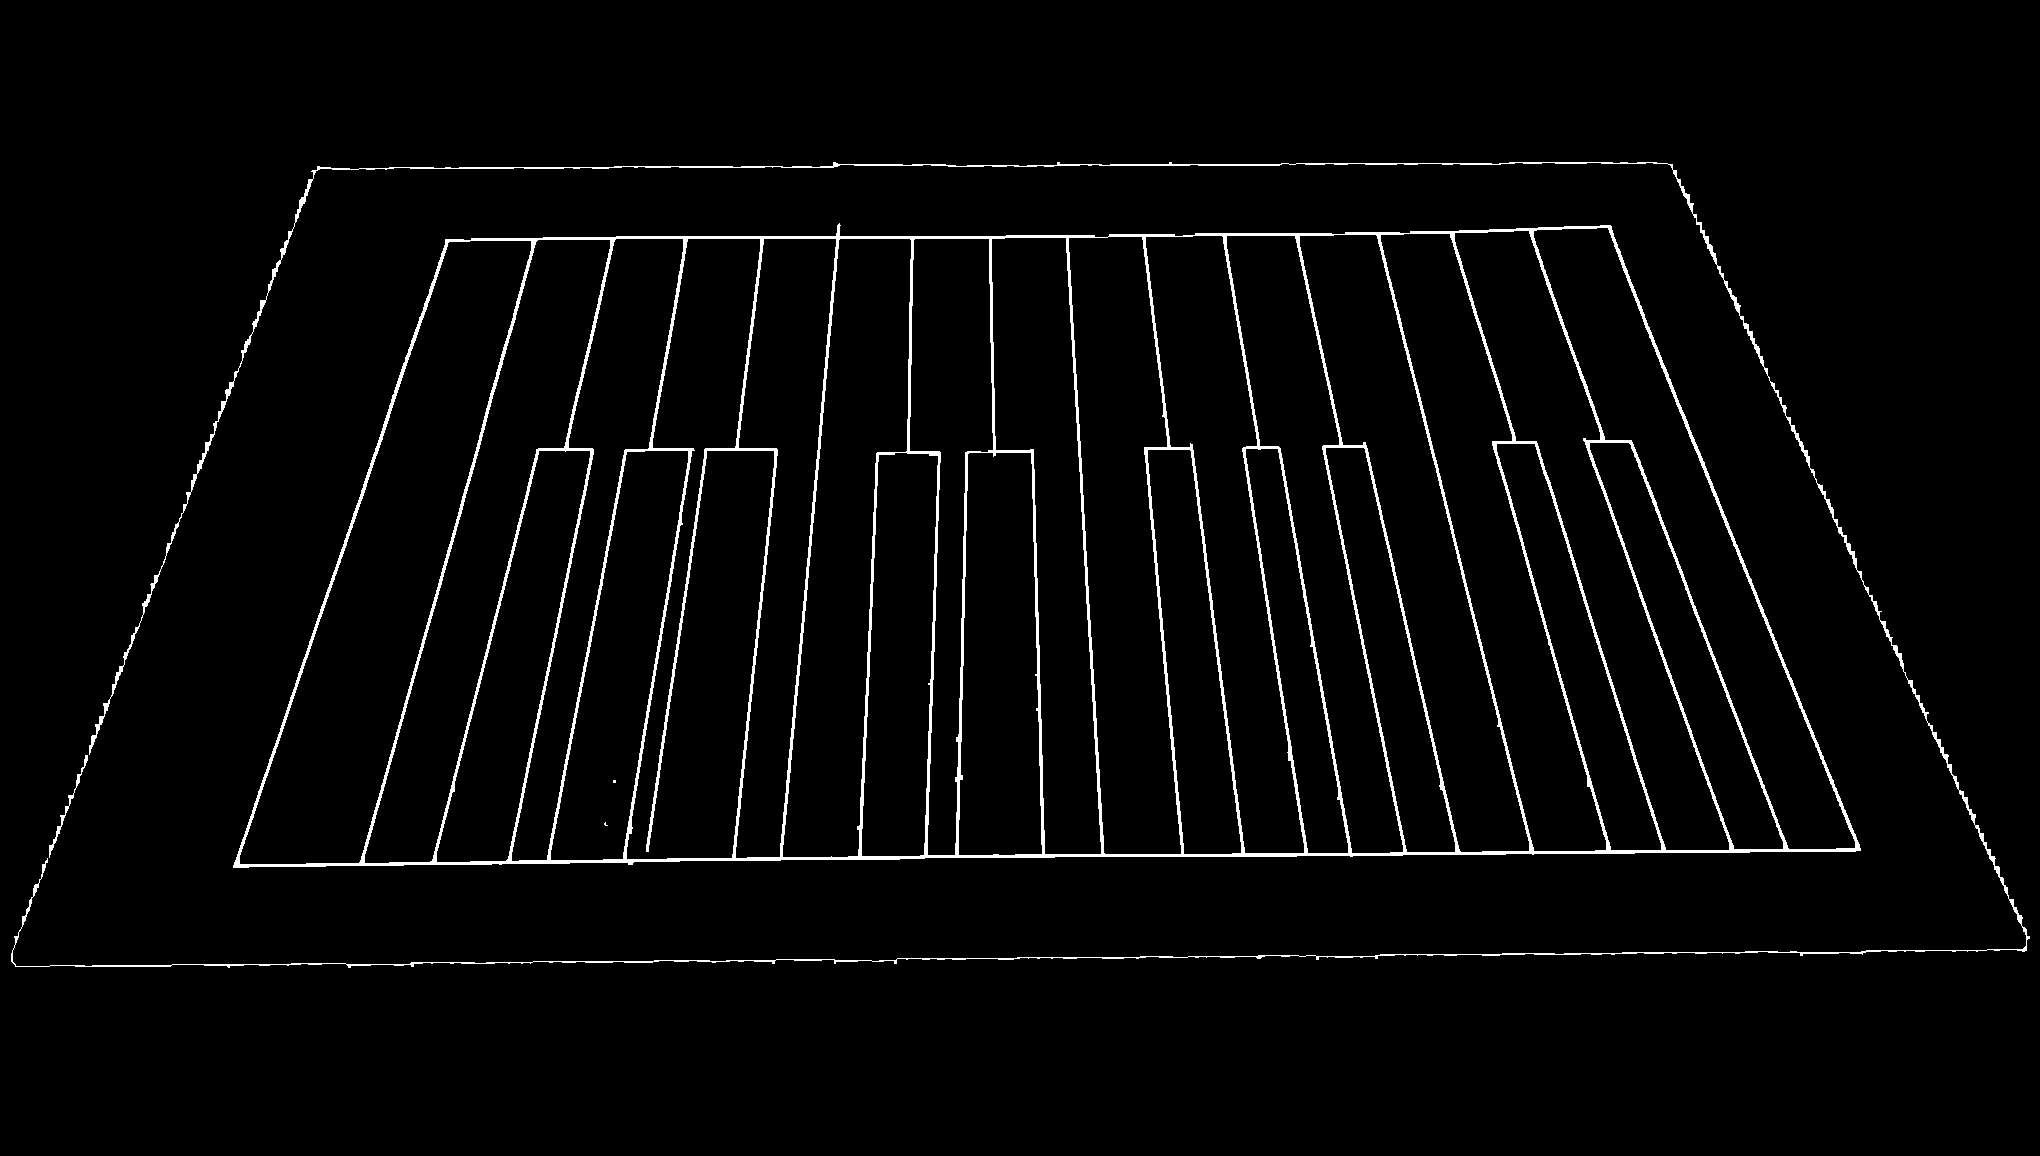
\includegraphics[width=\textwidth]{images/application/45deg/canny-closed}
		\caption{}
		\label{fig:canny-closed}
	\end{subfigure}
	\hfill
	\begin{subfigure}{0.49\textwidth}
		\centering
		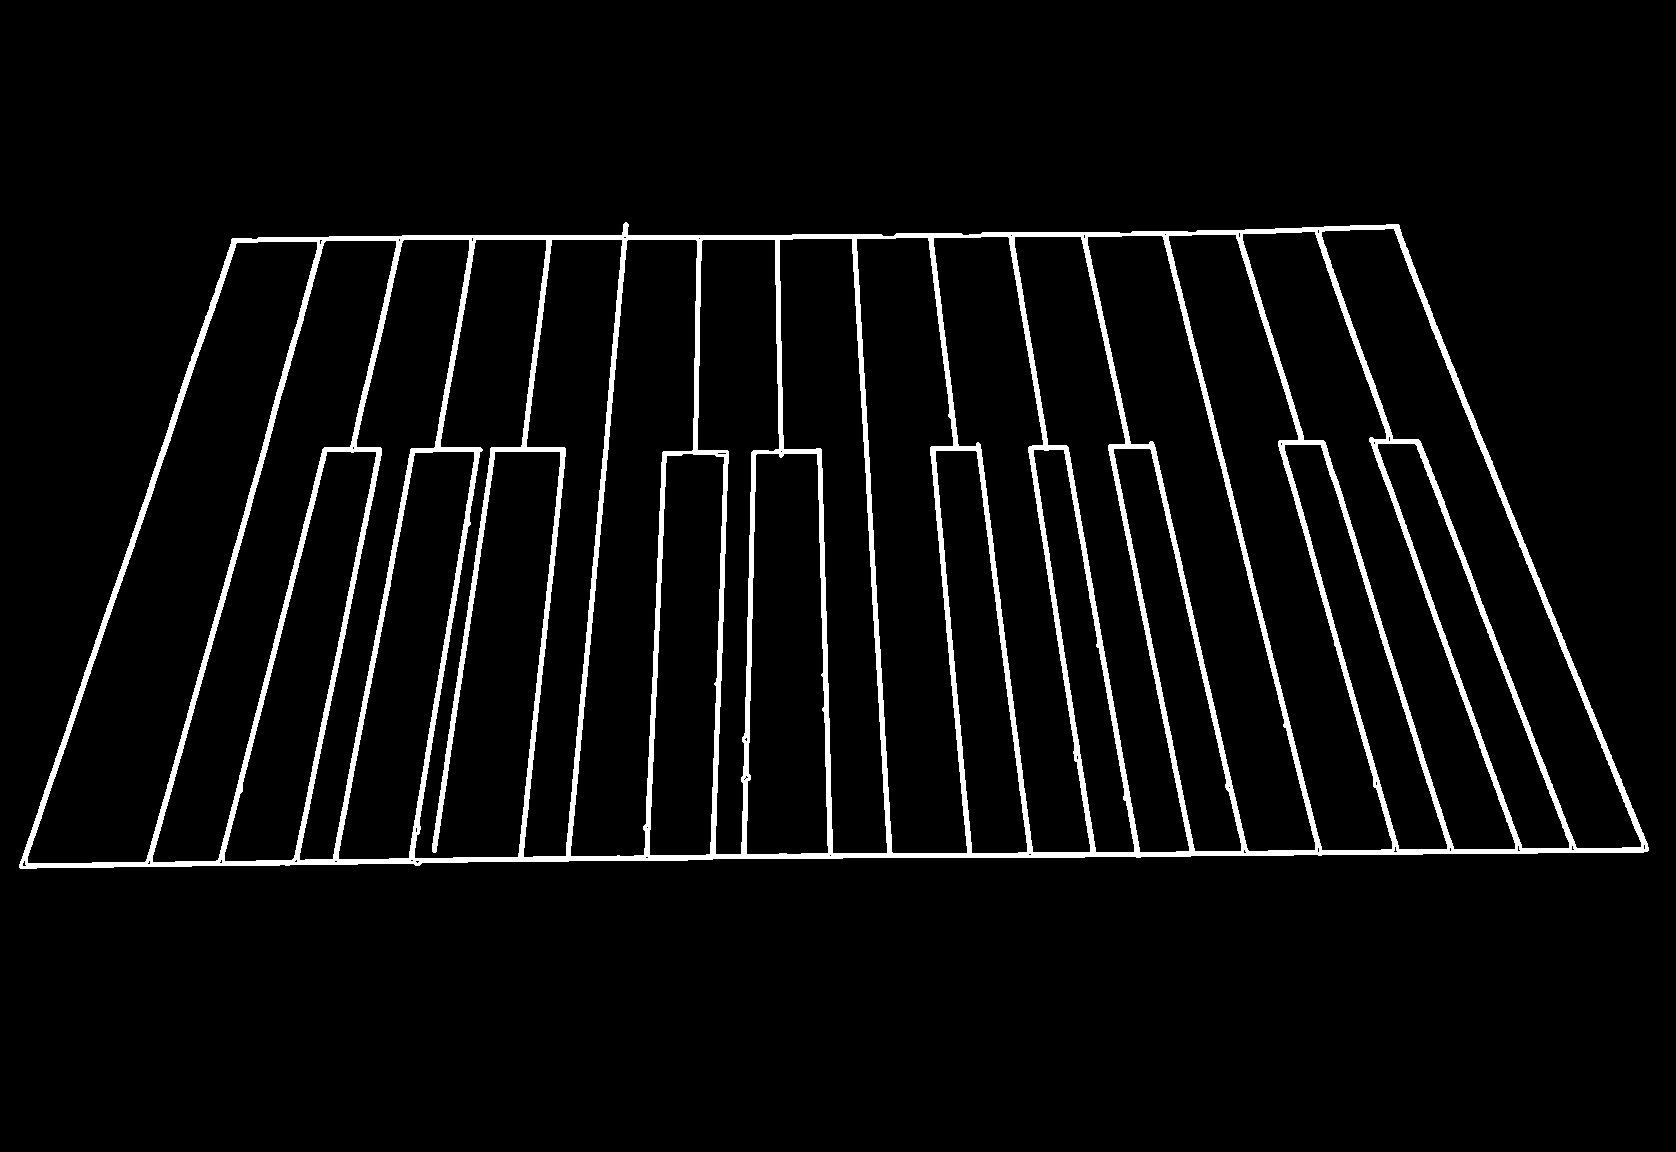
\includegraphics[width=\textwidth]{images/application/45deg/contours}
		\caption{}
		\label{fig:contours}
	\end{subfigure}
	\hfill
	\begin{subfigure}{0.49\textwidth}
		\centering
		\includegraphics[width=\textwidth]{images/application/45deg/tiles-overlay}
		\caption{}
		\label{fig:tiles-overlay}
	\end{subfigure}
	\hfill
	\begin{subfigure}{0.49\textwidth}
		\centering
		\includegraphics[width=\textwidth]{images/application/45deg/notes-overlay}
		\caption{}
		\label{fig:notes}
	\end{subfigure}
	\caption{
		Keyboard detection pipeline.
		(a) Perimeter;
		(b) Keyboard after background subtraction;
		(c) Canny edge;
		(d) Canny edge after morphological closure;
		(e) Contour detection (after filter);
		(f) Tiles overlay (not in transparency for visibility);
		(g) Notes indexes (brightness enhanced for visibility).
	}
	\label{fig:preprocessing}
\end{figure}

\subsubsection{Keyboard presets}
In this mode, instead of using a photo taken by the user to search for the keyboard and show the keys thus detected,
the shape and position of the keys that the application expects to use is shown directly.

The user can download and print out on an A4 sheet the model of the keyboard that the
application shows on the screen and must position it at the guides shown on the interface.
In this way, the user's physical keyboard will perfectly match the one presented by the application,
ensuring optimal performance and realism.

The PDF files for printing the keyboard presets will be available for download on the project's website.
The different keyboard models made available by default by the application are shown in \autoref{fig:presets}.

\begin{figure}[ht]
	\centering
	\begin{subfigure}{0.49\textwidth}
		\centering
		\includegraphics[width=\textwidth]{application/presets/keyboard-preset-1}
		\caption{}
		\label{fig:preset-1}
	\end{subfigure}
	\hfill
	\begin{subfigure}{0.49\textwidth}
		\centering
		\includegraphics[width=\textwidth]{application/presets/keyboard-preset-2}
		\caption{}
		\label{fig:preset-2}
	\end{subfigure}
	\caption{
		Keyboard presets different keyboard sizes.
		(a) One octave keyboard;
		(b) Two octaves keyboard.
	}
	\label{fig:presets}
\end{figure}


\subsection{Real-time phase}\label{subsec:real-time-phase}
When the user is satisfied with the result of the detection phase, they can press a button to start the real-time phase.
First, the graph is launched: the GPU manager is started, models for palm detection,
hand landmarks and handedness are loaded, and side packets are created.
Three data streams are started from the graph: \textit{hand landmarks}, \textit{world hand landmarks} and
\textit{handedness}, and an event listener is attached to each to receive the results of the processing of each frame.
The graph is schematised in \autoref{fig:mediapipe-graph}.

\begin{figure}[ht]
	\centering
	\includegraphics[width=\textwidth]{images/application/mediapipe-gpu}
	\caption{MediaPipe graph used in the application.}
	\label{fig:mediapipe-graph}
\end{figure}

The three data streams on which the outputs of the graph are passed work asynchronously
with respect to the main loop and also with respect to each other.
To ensure that the next step of the algorithm only starts when all three streams have produced a result
for the same frame, it was sufficient to implement a simple synchronisation system for the three outputs
to ensure that each frame is only passed to the next step of the algorithm when all three components are available.

Once all three components are available, our algorithm proceeds in its two phases:
\begin{itemize}
	\item \textit{Touch detection:} check if a finger touched the keyboard
	\item \textit{Note detection:} if a finger touched the keyboard,
	find which note was pressed and play the corresponding sound
\end{itemize}

It is important to note that, in its current state, not all three streams are used by our algorithm.
In particular, only the ones for \textit{hand landmarks} and \textit{handedness} are useful for our purposes.
The other, \textit{world hand landmarks}, is present mainly for reasons of compatibility with older
versions of the algorithm and the possibility that it will be useful in the future.

\paragraph{MediaPipe on low-end devices}
While the webcam and the video feed on the smartphone interface work at 30 FPS,
the frequency at which frames are sent to MediaPipe for hand detection is not fixed.
In order to meet all requirements and to be able to support as many smartphones as possible,
even low-end ones, we have implemented a way for the user to set the frequency at which frames are sent to
MediaPipe at will, i.e.\ the FPS at which the hand detection process runs.

This has been done by including buttons in the interface to directly increase and decrease the FPS with which to run MediaPipe.
Changing the value from the interface results in an immediate change in the operation of MediaPipe.

Through experimentation, we have found that a good value for MediaPipe's FPS is 15, which is high enough
to ensure that the app runs smoothly with low response times, but is not too high to be unusable on mid-range smartphones.

Going below 15 FPS is possible, but results in an increase in the app's response time and a possible loss of some notes.
Going above 15 FPS is also possible, and it is recommended in the case of high-end smartphones,
but being aware that increasing the frequency with which frames are sent to
MediaPipe also increases battery consumption and could lead to the smartphone overheating.

\subsubsection{Touch detection}
At this early stage of the project, the touch detection procedure is not yet very refined.
Since MediaPipe alone does not provide sufficiently precise depth coordinates (or camera distance) but rather
inconsistent and flickering ones, and for the reasons explained in \autoref{subsec:mp-for-3d}~\nameref{subsec:mp-for-3d},
we could not rely solely on them for the touch detection phase.
We therefore exploit the advantages explained in \autoref{subsec:pov}~\nameref{subsec:pov}.

To detect a touch, we rely on the position of the finger on the $y_s$ axis: when a finger reaches
down towards the paper to play a note, this movement is detected by MediaPipe thanks to the 45\degree \ view.
The $y_s$ position of the finger is given as input to an automaton that takes care
of maintaining and updating the state of the finger at each frame.
The automaton is illustrated in \autoref{fig:touch-automata}.

When a new frame is ready, the $x_s$ and $y_s$ positions of the finger are extracted from MediaPipe
and converted into pixels and the $y_s$ position is given to the automaton.
The automaton calculates the speed of the finger by comparing the new $y_s$ with the last detected $y_s$,
after which it advances the finger state accordingly.
When the finger enters the \textit{Touching} state, the $x_s$ and $y_s$ coordinates are passed to the note detector
which is responsible for verifying that the finger has touched a key and, if so, playing the corresponding note.
The automaton is made so that the \textit{Touching} state remains active even if the finger moves horizontally.

In \autoref{fig:touch-automata}, the \texttt{t} value indicates a threshold which serves to mitigate the instability of MediaPipe:
the hand landmarks detected by MediaPipe are subject to minute, continuous variations which, if not taken into account,
would cause a series of false positives and would repeatedly take the automaton in and out of the \textit{Touching} state.
Experimentally, we came to the conclusion that 8 is a suitable value for the automaton's activation threshold.

The pseudocode for this phase is shown in~\autoref{alg:touch-detection}.

\begin{algorithm}
	\caption{Touch detection}
	\begin{algorithmic}[1]
		\State when new frame arrives
		\If{no hand has been detected}
			\State \Return
		\EndIf
		\State $toPlay \gets \{\}$
		\For{each hand $h$ detected}
			\For{each finger $f$ of $h$}
				\State $x \gets$ horizontal position of $f$
				\State $y \gets$ vertical position of $f$
				\State $isPlaying \gets$ automata($f$).update($y$)
				\If{$isPlaying$}
					\State $toPlay \gets toPlay \ \bigcup \ \left\{ \left( x, y \right) \right\}$
				\EndIf
			\EndFor
		\EndFor
		\State do \textit{note detection} with $toPlay$
	\end{algorithmic}
	\label{alg:touch-detection}
\end{algorithm}

\begin{figure}[ht]
	\centering
	\includegraphics[width=\textwidth]{images/application/touch-automata}
	\caption{The automata used to detect finger touch.}
	\label{fig:touch-automata}
\end{figure}

\subsubsection{Note detection}\label{subsubsec:notes-detection}
Once we have detected the fingers touching the keyboard with MediaPipe,
we need to work out which notes have been touched.
To do this, we use the image generated in the keyboard detection phase in
\autoref{par:notes-detection}~\nameref{par:notes-detection}.

This image is the same size as the video feed and is totally black except where the keys are located.
The keys are coloured in a grey scale where the first key is coloured with the value 1,
the second with the value 2 and so on.
This allows us to associate each key with a unique value that we can use to determine the note to be played.

Using the $x_s$ and $y_s$ coordinates provided by MediaPipe, we can superimpose them on the image generated
in the keyboard detection phase to determine whether a finger has touched a key.
If the pixel at position $(x, y)$ is black, the finger is outside the keyboard and nothing happens.
If, on the other hand, the pixel is not black, the finger is on one of the detected keys and therefore the MIDI signal
corresponding to the detected note at that position must be played.

Playing sounds is not as straightforward a process as it might seem, and it does require a little forethought.
This is because when passing from one frame to another, some fingers that were playing
in the previous frame may still be playing the same key.
In this case the note does not have to be played again, but only continued.

To do this, we keep a list of the notes that are being played and, at each frame, create two different sets of notes:
the set of notes that were being played in the previous frame but are no longer being played in the current frame,
and the set of notes that were not being played in the previous frame but are being played in the current frame.

This allows to detect notes that were being played in the previous frame and are still being played in the current frame,
so that they are not played again but remain playing.

The pseudocode for this phase is shown in~\autoref{alg:note-detection}.

\begin{algorithm}
	\caption{Note detection}
	\begin{algorithmic}[1]
		\State \textbf{Input}: the set of coordinates $toPlay$ of the fingers touching the keyboard
		\State $playing \gets \{n \ | \ n \text{ is already being played from the previous frame}\}$
		\State $detected \gets \{ n \ | \ (x, y) \in toPlay \text{ and }\newline
		\hspace*{21.6mm} n \text{ is a non-black pixel at } (x, y) \text{ in the note image}\}$
		\State $stop \gets playing \setminus detected$
		\State $start \gets detected \setminus playing$
		\For{each $n$ in $stop$}
			\State stop playing note $n$
		\EndFor
		\For{each $n$ in $start$}
			\State start playing note $n$
		\EndFor
	\end{algorithmic}
	\label{alg:note-detection}
\end{algorithm}

\begin{figure}[ht]
	\centering
	\includegraphics[width=\textwidth]{images/application/screenshots/detection-phase}
	\caption{Application during detection phase, with perimeter visible.}
	\label{fig:screenshot-detection-phase}
\end{figure}

\begin{figure}[ht]
	\centering
	\includegraphics[width=\textwidth]{images/application/screenshots/playing-phase}
	\caption{Application after keyboard detection, with keyboard overlay visible.}
	\label{fig:screenshot-playing-phase}
\end{figure}




	\chapter{Results}\label{ch:results}
In this chapter, we present the findings from the experiments conducted to evaluate the performance
and usability of the mixed reality musical keyboard application, Keyrtual.
The results are structured into two primary sections: quantitative results, which measure the technical performance
of the keyboard detection and real-time interaction processes, and qualitative results,
which assess user feedback based on perceived ease of use and experience.
Through these experiments, we aim to establish the effectiveness of the application
and highlight areas for further development.

\section{Quantitative results}\label{sec:quantitative-results}
The experiments carried out on the application concern the two fundamental
phases of the pipeline: the keyboard detection phase and the real-time phase.

\subsection{Keyboard detection}\label{subsec:keyboard-detection}
Experiments to evaluate the keyboard detection algorithm were carried out on 3 different types of keyboard:
a hand-drawn keyboard, a keyboard drawn with a ruler as the one shown in~\autoref{fig:screenshot-detection-phase},
and a keyboard printed using the preset provided by the application shown in~\autoref{fig:preset-1}.

The tests were carried out in a room with artificial light coming from the ceiling
and natural light coming from an open window.
For each of these keyboards, the test was carried out by changing the rotation and position of
the keyboard with respect to the natural light 4 times, performing the keyboard detection 3 times for each position,
for a total of 12 detections per keyboard type and 36 detections in total.

The evaluation of the experiments consists of comparing the result obtained from the keyboard detection, such as the
one shown in~\autoref{fig:tiles-overlay}, with the optimal result we would expect to obtain from a perfect detector.
Of course, we are not able to obtain the optimal result with an algorithm,
otherwise we would use that same algorithm to do the detection.
So to create the ground truth we used a photo editing software to manually colour
in black and white exactly the spaces occupied by the keys.

Once we had created the ground truth for all 36 photos,
we applied the keyboard detection algorithm to each of them and compared it to the ground truth
by doing a simple subtraction of colours to highlight individual differing pixels.
To calculate the pixel accuracy of our detection algorithm we used the following formula
\[
	Accuracy = \frac{TP}{n}
\]
where $TP$ (true positives) is the number of pixels correctly classified by the algorithm and $n$ is the total number
of pixels within the area bounded by the perimeter, as can be seen in~\autoref{fig:screenshot-detection-phase}.
We used the number of pixels inside the perimeter and not the total number of pixels in the image because doing so
would have produced higher but untrue percentages, as the algorithm only searches for the keyboard in
the area of the image bounded by the perimeter and not in the entire image.

As can be seen in~\autoref{tab:keyboard-detection-accuracy},
the results for the detection algorithm are excellent for each type of keyboard.

\begin{table}[ht]
	\centering
	\begin{tabular}{l|l|}
		\cline{2-2}
		& Pixel accuracy               \\ \hline
		\multicolumn{1}{|l|}{Hand-drawn}       & \multicolumn{1}{c|}{95.00\%} \\ \hline
		\multicolumn{1}{|l|}{Drawn with ruler} & \multicolumn{1}{c|}{96.74\%} \\ \hline
		\multicolumn{1}{|l|}{Printed}          & \multicolumn{1}{c|}{97.69\%} \\ \hline
	\end{tabular}
	\caption{Pixel accuracy of keyboard detection algorithm}
	\label{tab:keyboard-detection-accuracy}
\end{table}

Unfortunately, we did not conduct the same experiment for the keyboard detection algorithm in the old prototype,
so we cannot compare the results.
However, based on our experience with both algorithms,
we can state with absolute certainty that the new algorithm is much better performing than the old one,
which was only able to detect straight lines, needed the additional step of background subtraction,
and didn't even produce a visible result like the new one does.

\subsection{Real-time phase}\label{subsec:real-time-phase-results}
To evaluate the real-time phase we used a method similar to the one used in the old prototype:
we played a series of notes on the keyboard and counted the times in which the application reacted correctly or not.

In order to evaluate the performance of the application's real-time phase according to its accuracy,
precision, and recall, we needed to calculate the amount of true positives ($TP$), true negatives ($TN$),
false positives ($FP$) and false negatives ($FN$).
The meaning of these terms in our application is schematized in~\autoref{tab:tp-tn-fp-fn}.

\begin{table}[ht]
	\centering
	\begin{tabular}{l|l|l|}
		\cline{2-3}
		& User plays                & User does not play        \\ \hline
		\multicolumn{1}{|l|}{Application plays}         & \multicolumn{1}{c|}{$TP$} & \multicolumn{1}{c|}{$FP$} \\ \hline
		\multicolumn{1}{|l|}{Application does not play} & \multicolumn{1}{c|}{$FN$} & \multicolumn{1}{c|}{$TN$} \\ \hline
	\end{tabular}
	\caption{Meaning of $TP$, $TN$, $FP$ and $FN$ in our application}
	\label{tab:tp-tn-fp-fn}
\end{table}

To achieve the maximum precision in calculating these values, we modified the real-time algorithm to be able to save
each frame associated with a label indicating whether in that frame the algorithm detected a touch or not.
After the recording, we manually checked each frame with the corresponding label and counted if it was a $TP$, $TN$, $FP$ or $FN$.

In this way we carried out 3 experiments.
In each experiment the user had to press a finger on all the keys of the keyboard in order from left to right.
The results of the experiments are shown in~\autoref{tab:real-time-results},
together with the results from the old prototype.

\begin{table}[ht]
	\centering
	\begin{tabular}{c|c|c|c|c|}
		\cline{2-5}
		& Accuracy                      & Precision                     & Recall                        & F$_1$                         \\ \hline
		\multicolumn{1}{|l|}{Old prototype} & \multicolumn{1}{|c|}{90.27\%} & \multicolumn{1}{|c|}{56.87\%} & \multicolumn{1}{|c|}{99.40\%} & \multicolumn{1}{|c|}{72.35\%} \\ \hline
		\multicolumn{1}{|l|}{New version}   & \multicolumn{1}{|c|}{87.40\%} & \multicolumn{1}{|c|}{80.23\%} & \multicolumn{1}{|c|}{81.18\%} & \multicolumn{1}{|c|}{80.70\%} \\ \hline
	\end{tabular}
	\caption{Comparison of real-time phase between old prototype and current version}
	\label{tab:real-time-results}
\end{table}

The comparison between the old and the new version highlights how the real-time phase of the application is now much
more precise than before, and on average more stable and reliable.
The recall of the new version is much lower than before, but this is because in the old version there were very few
false negatives thanks to the presence of the Leap Motion Controller.


\section{Qualitative results}\label{sec:qualitative-results}
We also retrieved results about the perceived usability of our application with the same method used for the old prototype.
We asked 15 participants to play with the application for 5 minutes,
from the keyboard detection phase to the playing phase, and to fill out the UMUX questionnaire
(Usability Metric for User Experience~\cite{umux}) at the end.
Among the participants involved in the experiment, there were people with different musical background knowledge:
6 had no musical knowledge at all, 6 had little musical knowledge mainly from middle school and high school,
and 3 were professional piano players.

The results of the questionnaire are shown in~\autoref{tab:usability-results},
together with the results from the old prototype.

\begin{table}[ht]
	\centering
	\begin{tabular}{l|l|l|l|}
		\cline{2-4}
		& Minimum                       & Average                       & Maximum                       \\ \hline
		\multicolumn{1}{|l|}{Old prototype} & \multicolumn{1}{|c|}{70.83\%} & \multicolumn{1}{|c|}{79.86\%} & \multicolumn{1}{|c|}{87.50\%} \\ \hline
		\multicolumn{1}{|l|}{New version}   & \multicolumn{1}{|c|}{84.11\%} & \multicolumn{1}{|c|}{92.28\%} & \multicolumn{1}{|c|}{97.91\%} \\ \hline
	\end{tabular}
	\caption{Comparison of usability between old prototype and current version}
	\label{tab:usability-results}
\end{table}

These results highlight how the porting from computer to smartphone,
the elimination of all additional hardware, and the simplification of the keyboard detection procedure
have greatly improved the usability and portability of the entire system.



	\chapter{Conclusions}\label{ch:conclusions}
In this work, progress was made on the creation of a mixed reality application dedicated to
teaching music in schools, especially in the first approach to the subject.
The work starts with an existing prototype, which had the shortcoming of requiring a computer and specific hardware
to run, and brings it to a mobile device, a smartphone, accessible to all and available at affordable prices.
The software can also run without problems on cheap and not too recent devices,
while still achieving performance similar to that of top-of-the-range devices.

The biggest improvements were found in the general usability of the application, thanks to the porting to smartphones
and the elimination of all external hardware, and in the keyboard detection algorithm,
which achieves almost perfect results on any type of keyboard without the need for any special lighting measures
and now consists of a single step.

Some progress was made also in the playing phase, which is now more precise and reliable on average,
but there is still much room for improvement.


\section{Future development}\label{sec:future-development}
In the next stages of development we plan to improve the touch recognition algorithm
to achieve better precision and accuracy.
This will be done by completely changing the keyboard detection phase from the current single-shot phase to a slightly
longer procedure, but one that we hope will lead to better results.

The idea is to use plane detection techniques to locate the table with the paper on it, do the keyboard detection
from above, and then move the phone to a very low angle, almost parallel to the table, tracking the position of the
paper (and thus the keyboard) in 3D space while the phone moves to the new position.

This would allow us to have a perfect view of the distance of the fingers from the sheet, greatly increasing the
accuracy of touch recognition, while maintaining full information on the position of the keys thanks to plane
detection and tracking of the sheet during the transition from 90\degree \ to the flat position.

Plane detection and keyboard tracking can be made very accurate by the fact that the size of the sheet is known,
being an ordinary A4 sheet.
View from the flat position is shown in~\autoref{fig:future-work}.

As an alternative to the above strategy, it would be possible to develop an ad-hoc neural network,
suitable for running on mobile devices, with the aim of detecting, from the RGB image alone,
which fingers are pressed on the surface of the sheet.
This neural network, if developed, will be trained with a dataset of images of hands in different positions and with
different fingers pressed, and will be able to return, for each frame, which fingers are pressed and on which keys.

We also plan to assess the feasibility of porting it to iOS, to expand the pool of users that our application can reach.

\begin{figure}[ht]
	\centering
	\includegraphics[width=\textwidth]{images/application/screenshots/playing-phase-flat}
	\caption{Flat view of the keyboard, still in development.}
	\label{fig:future-work}
\end{figure}


	\backmatter
	\cleardoublepage
	\phantomsection
	\addcontentsline{toc}{chapter}{\bibname}
	\bibliographystyle{sapthesis}
	\bibliography{bibliography}

\end{document}
